%%%% Proceedings format for most of ACM conferences (with the exceptions listed below) and all ICPS volumes.
\documentclass[sigconf, authordraft]{acmart}
%%%% As of March 2017, [siggraph] is no longer used. Please use sigconf (above) for SIGGRAPH conferences.

%%%% Proceedings format for SIGPLAN conferences 
% \documentclass[sigplan, anonymous, review]{acmart}

%%%% Proceedings format for SIGCHI conferences
% \documentclass[sigchi, review]{acmart}

%%%% To use the SIGCHI extended abstract template, please visit
% https://www.overleaf.com/read/zzzfqvkmrfzn

\usepackage{booktabs} % For formal tables


% Copyright
%\setcopyright{none}
%\setcopyright{acmcopyright}
%\setcopyright{acmlicensed}
\setcopyright{rightsretained}
%\setcopyright{usgov}
%\setcopyright{usgovmixed}
%\setcopyright{cagov}
%\setcopyright{cagovmixed}


% DOI
\acmDOI{10.475/123_4}

% ISBN
\acmISBN{123-4567-24-567/08/06}

%Conference
\acmConference[WOODSTOCK'97]{ACM Woodstock conference}{July 1997}{El
  Paso, Texas USA}
\acmYear{1997}
\copyrightyear{2016}

\acmPrice{15.00}

\acmSubmissionID{123-A12-B3}

\begin{document}
\title{SIG Proceedings Paper in LaTeX Format}
\titlenote{Produces the permission block, and
  copyright information}
\subtitle{Extended Abstract}
\subtitlenote{The full version of the author's guide is available as
  \texttt{acmart.pdf} document}


\author{Ben Trovato}
\authornote{Dr.~Trovato insisted his name be first.}
\orcid{1234-5678-9012}
\affiliation{%
  \institution{Institute for Clarity in Documentation}
  \streetaddress{P.O. Box 1212}
  \city{Dublin}
  \state{Ohio}
  \postcode{43017-6221}
}
\email{trovato@corporation.com}

\author{G.K.M. Tobin}
\authornote{The secretary disavows any knowledge of this author's actions.}
\affiliation{%
  \institution{Institute for Clarity in Documentation}
  \streetaddress{P.O. Box 1212}
  \city{Dublin}
  \state{Ohio}
  \postcode{43017-6221}
}
\email{webmaster@marysville-ohio.com}

\author{Lars Th{\o}rv{\"a}ld}
\authornote{This author is the
  one who did all the really hard work.}
\affiliation{%
  \institution{The Th{\o}rv{\"a}ld Group}
  \streetaddress{1 Th{\o}rv{\"a}ld Circle}
  \city{Hekla}
  \country{Iceland}}
\email{larst@affiliation.org}

\author{Lawrence P. Leipuner}
\affiliation{
  \institution{Brookhaven Laboratories}
  \streetaddress{P.O. Box 5000}}
\email{lleipuner@researchlabs.org}

\author{Sean Fogarty}
\affiliation{%
  \institution{NASA Ames Research Center}
  \city{Moffett Field}
  \state{California}
  \postcode{94035}}
\email{fogartys@amesres.org}

\author{Charles Palmer}
\affiliation{%
  \institution{Palmer Research Laboratories}
  \streetaddress{8600 Datapoint Drive}
  \city{San Antonio}
  \state{Texas}
  \postcode{78229}}
\email{cpalmer@prl.com}

\author{John Smith}
\affiliation{\institution{The Th{\o}rv{\"a}ld Group}}
\email{jsmith@affiliation.org}

\author{Julius P.~Kumquat}
\affiliation{\institution{The Kumquat Consortium}}
\email{jpkumquat@consortium.net}

% The default list of authors is too long for headers.
\renewcommand{\shortauthors}{B. Trovato et al.}


\begin{abstract}
This paper provides a sample of a \LaTeX\ document which conforms,
somewhat loosely, to the formatting guidelines for
ACM SIG Proceedings.\footnote{This is an abstract footnote}
\end{abstract}

%
% The code below should be generated by the tool at
% http://dl.acm.org/ccs.cfm
% Please copy and paste the code instead of the example below.
%
\begin{CCSXML}
<ccs2012>
 <concept>
  <concept_id>10010520.10010553.10010562</concept_id>
  <concept_desc>Computer systems organization~Embedded systems</concept_desc>
  <concept_significance>500</concept_significance>
 </concept>
 <concept>
  <concept_id>10010520.10010575.10010755</concept_id>
  <concept_desc>Computer systems organization~Redundancy</concept_desc>
  <concept_significance>300</concept_significance>
 </concept>
 <concept>
  <concept_id>10010520.10010553.10010554</concept_id>
  <concept_desc>Computer systems organization~Robotics</concept_desc>
  <concept_significance>100</concept_significance>
 </concept>
 <concept>
  <concept_id>10003033.10003083.10003095</concept_id>
  <concept_desc>Networks~Network reliability</concept_desc>
  <concept_significance>100</concept_significance>
 </concept>
</ccs2012>
\end{CCSXML}

\ccsdesc[500]{Computer systems organization~Embedded systems}
\ccsdesc[300]{Computer systems organization~Redundancy}
\ccsdesc{Computer systems organization~Robotics}
\ccsdesc[100]{Networks~Network reliability}


\keywords{ACM proceedings, \LaTeX, text tagging}


\maketitle

\section{Introduction}\label{Introduction}
In software development, the reuse of existing software artifacts has been explored for decades \cite{mussbacher2013vision,krueger1992software,nato}, including but not limited to classes, components \cite{harsh2006component}, design patterns \cite{gangoffour}, frameworks \cite{johnson1997frameworks}, Software Product Lines \cite{pohl2005software}, and Reusable Aspect Models (RAM) \cite{kienzle2009aspect}. Every programming language has numerous software libraries to facilitate reuse. Software reuse can increase the productivity, software quality and minimize development cost, time-to-market and schedule overruns \cite{kim1998software}.  In general, any software artifact can be reused. Although, there are numerous benefits of software reuse, the efforts required to reuse a software artifact should not outweigh those required to create the software system from scratch. Therefore, there is an imperative need to streamline the reusability of software artifacts.

Owing to the advent of model driven engineering \cite{brambilla2012model, schmidt}, virtually all software artifacts can be represented as models including reusable artifacts. While great efforts have been made to increase the reusability of software models, little or no work\footnote{A search in the IEEE Xplore and ACM Digital Libraries for publications at the MODELS conference and the search term "layout" \haAction{and in Google Scholar, with the search terms: "layout merge" and "layout merging"} resulted in only eight relevant publications which are discussed further in Section \ref{RW}. However, none of them addresses the layout of reused models.}\label{f1} has been done to improve the resulting layout when combining a reusing and reused model. For some modeling languages, the layout of the resulting model composed of the reusing and reused model does not pose a challenge. In behavioral models, the reusing model often simply references the reused model. For other models such as Feature Models \cite{kang1990feature}, the layout is straightforward even for composed models. However, other modeling languages require the merging of model elements in the reusing and reused models as is the case for many structural models and particularly aspect-oriented techniques (e.g., Kompose \cite{komposeOnline}, Theme/UML \cite{themeuml}, and RAM \cite{kienzle2009aspect}) and more generally model transformations with the intent \cite{lucio2016model} to merge structural models (e.g., MATA \cite{mata}). 

State-of-the-art layout mechanisms used to layout models, e.g., GraphViz \cite{graphviz} and JGraphX \cite{JgraphX}, do not retain the original layout information and rather arbitrarily layout the merged models. However, the specific layout of a model often conveys important information \cite{misue1995layout}, which is currently lost with the existing mechanisms. This paper addresses this problem by establishing a robust layout algorithm called rpGraph which aims to retain the layout information of reusing and reused models when they are combined. As a representative, we use RAM to demonstrate rpGraph in this work, but our findings are also applicable to other merge-based techniques. In RAM, class diagrams are used to describe artifacts which are combined during reuse. The aim is to retain the general topology of the individual class diagrams, i.e., the reusing and reused models, to maintain the \textit{modeler's mental map} \cite{misue1995layout,von2007mental}.

As a prerequisite for rpGraph, we assume that the reused and reusing models have a proper, desired layout formulated by the modeler. The main contributions of this work are\haAction{:} \haReplace{First, we present a layout metamodel which can be used to graphically represent models based on their relative positioning with the help of automatic layout mechanisms such as GraphViz. This can be applied not only in model reuses but also in model adjustment \cite{misue1995layout, gregorics2015textual, incrementaldiagram}. Second, we present a layout algorithm that largely retains the layout of models when merged during reuse.}{
\haDeleted{ twofold.} 
\begin{enumerate}
\item We present metrics to compare layout diagrams and used it in evaluation of our algorithm against other layout mechanisms, GraphViz and JGraphX.
\item We present a layout metamodel which can be used to graphically represent models based on their relative positioning with the help of automatic layout mechanisms such as GraphViz. This can be applied not only in model reuses but also in model adjustment \cite{misue1995layout, gregorics2015textual, incrementaldiagram}. 
\item We present a layout algorithm that largely retains the layout of models when merged during reuse.
\item Finally, we apply rpGraph to Concern Oriented Reuse layout of models.
\end{enumerate}
}
   
Our findings are evaluated with 20 example model reuses from a library of reusable software model artifacts. In each case, two models with proper layout are combined and the layout of the combined model is compared against the original models. In this work, rpGraph, GraphViz (Graph Visualization Software), and JGraphX  (the approach currently used by the RAM tool TouchCORE) layout visualizations are used to layout the merged models and the topology of each layout is compared against the others. \haAction{We further apply rpGraph to Concern Oriented Reuse (CORE) as a case study and the results of the merged models are also compared against GrapgViz and JGraphX.} Overall, rpGraph performs better in retaining the structure of the original models. \haAction{The adjacent positions of nodes in each layout diagram are maintained after the diagrams are merged while other layout mechanisms disorient the positioning after merging.}  

In the remainder of this paper, we first present the motivation and background of the study in Section \ref{background}. Section \ref{related work} discusses related work while Section \ref{The work} presents the metamodel and the algorithm of rpGraph. In Section \ref{discussion}, we present \haAction{the layout comparison metrics }and discuss the resulting layout of rpGraph and compare it against GraphViz and JGraphX. \haAction{Section \ref{core} discusses Concern Oriented Reuse while we present and discuss the resulting layouts of CORE diagrams in Section \ref{concern discussion}. Section \ref{threats to validity} presents threats to validity of our study.} The conclusion in Section \ref{conclusion} summarizes the contributions of the study and presents future work.

\section{Background} \label{background}
This section presents a motivating example as well as background information on how models are reused with RAM and the TouchCORE tool.

\subsection{Model Reuses with Concerns} \label{concern reuse}
Software reuse is defined as the process of creating new software systems using existing software artifacts rather than creating them from scratch \cite{krueger1992software}. A concern is a generic unit of reuse which groups related models (e.g., class diagrams, sequence diagrams, state machines) that cut across software application \cite{alam2013concern}. \haAction{These related artifacts are grouped using the concept of Software Product Line \cite{spl}, which expresses the commonalities and variabilities among the software artifacts. Each artifact can be described using difference modeling diagram including class diagram, sequence diagram, use case diagram, or activity diagram.} Examples of concerns are authentication, authorization, and logging. In this paper, we focus on concerns and in particular class diagrams specified with Reusable Aspect Model (RAM) \cite{alam2013concern} to describe the structural dimension of a concern. Each concern provides three interfaces to facilitate reuse: the variation, customization, and usage interfaces. 

\haReplace{
The variation interface describes provided features of the concern and their impact on system qualities. The customization interface allows adapting a chosen variation of the concern to a specific reuse context, while the usage interface defines how a customized concern may eventually be used \cite{alam2016concern}.   
}{
\subsubsection{Variation Interface:} The \textit{variation interface} specifies the variabilities and commonalities in a family of software artifacts that a concern provides and the impact of each selection on system qualities. This helps a software designer to tailor a given concern to her specific needs via selection of different artifacts.
\subsubsection{Customization Interface:} The \textit{customization interface} allows adapting a chosen variation of the concern to a specific reuse context. For example, a concept Authenticatable, in an authentication concern is adapted or customized as a User in a bank application.
\subsubsection{Usage Interface:} The \textit{usage interface} defines how a customized concern may eventually be used \cite{alam2016concern}. It specifies the design structure and behaviour that the concern provides to the reusing application. In class diagram, the usage interface is the set of all public class properties, i.e., the attributes and the operations that are visible and accessible from the rest of the application.}

\begin{figure*}
	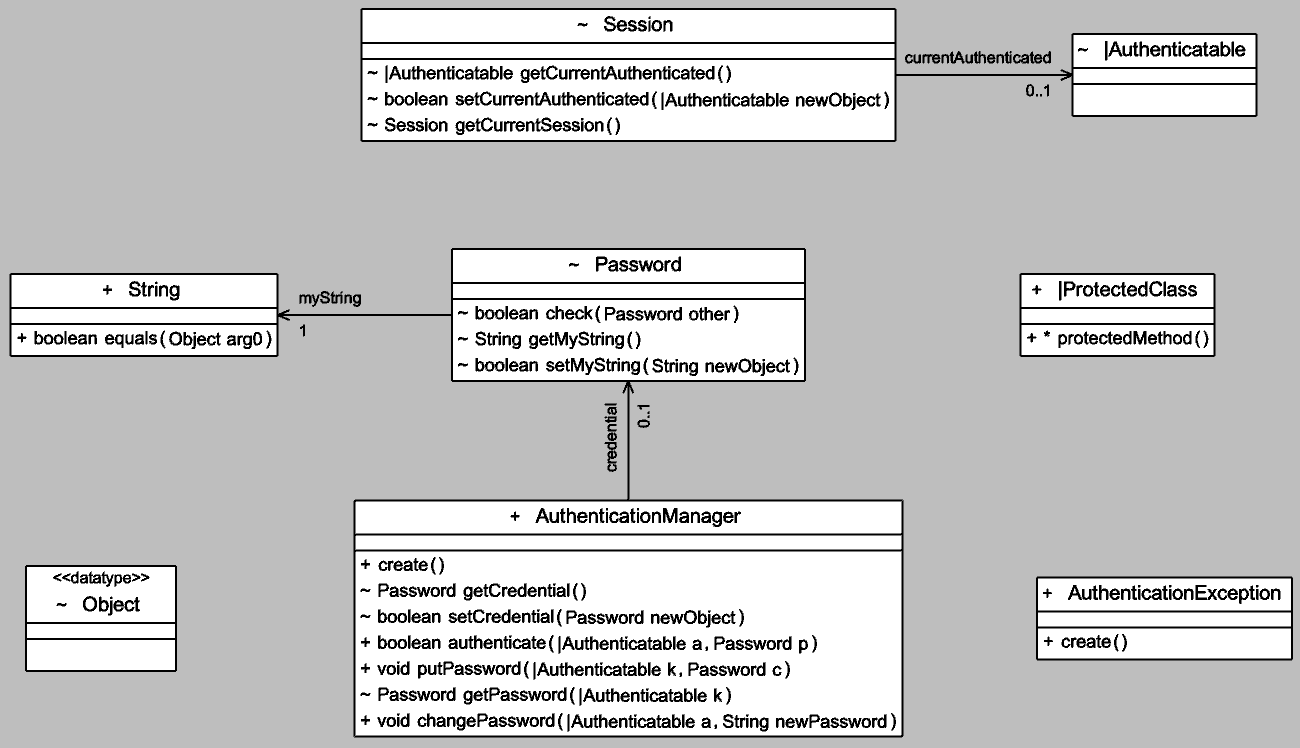
\includegraphics[width=\linewidth, height = 8cm]{authentication.PNG}
	\caption{Authentication concern}
	\label{fig :Authentication Concern}
\end{figure*}
\begin{figure}
	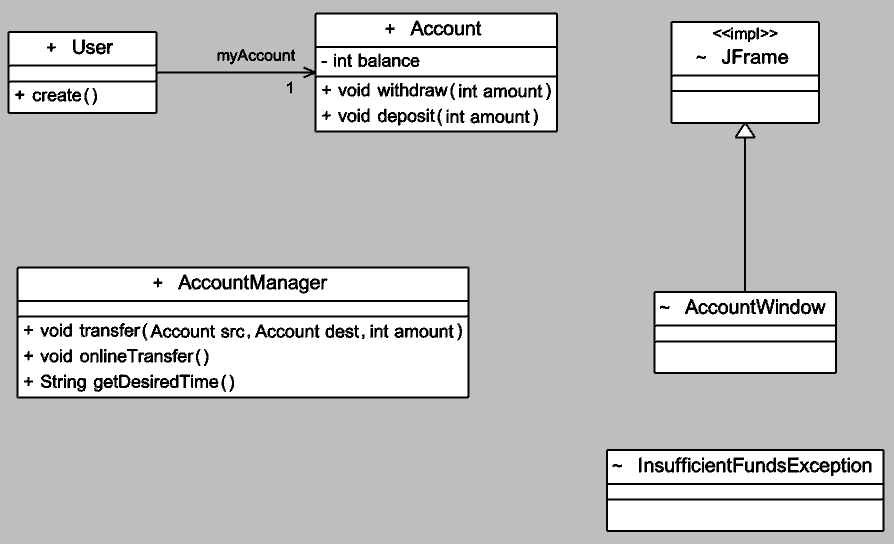
\includegraphics[width=\linewidth]{bank.PNG}
	\caption{Bank application}
	\label{fig :Bank App}
\end{figure}
\begin{figure*}
	\centering
    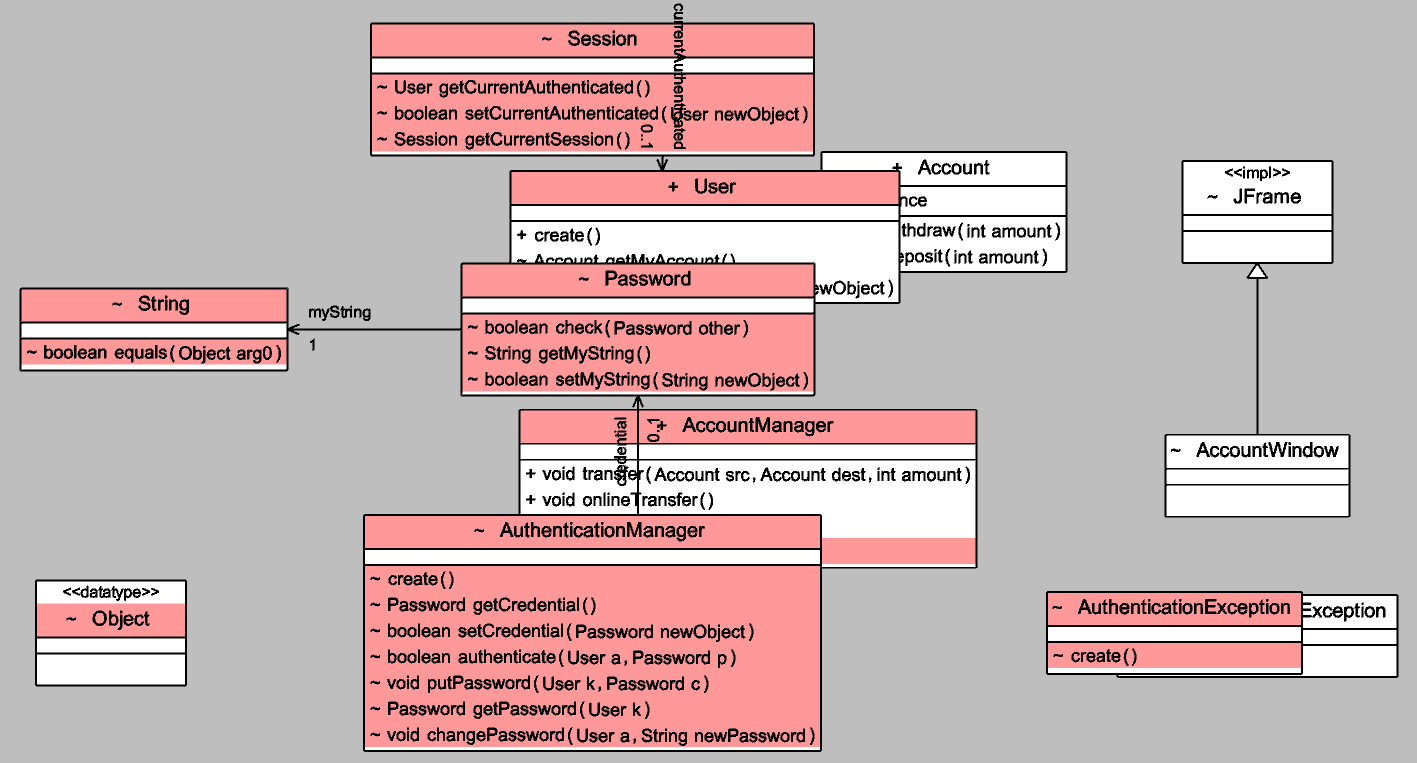
\includegraphics[width=\linewidth]{default_bank.PNG}
    \caption{\haDeleted{Default layout of} Merged model of bank and authentication}
    \label{fig : default bank and authentication}
\end{figure*}
\begin{figure*}
    	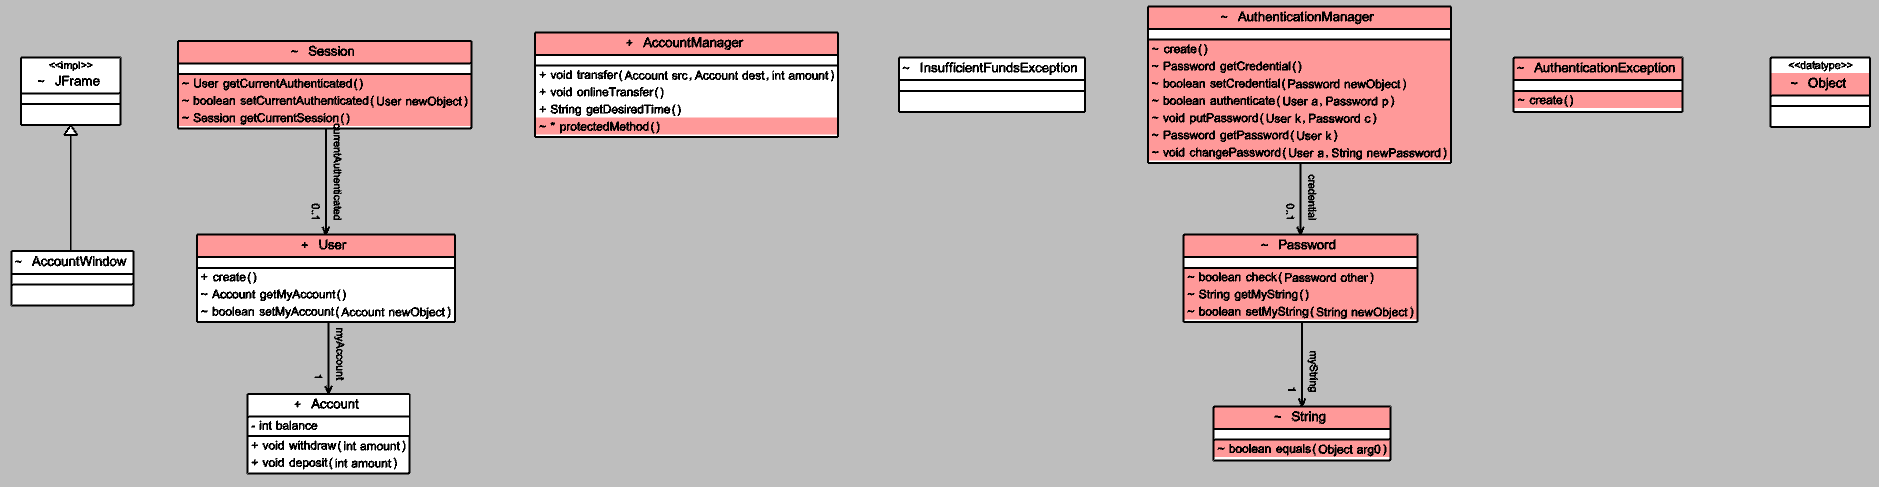
\includegraphics[width=\linewidth]{gv_bank.PNG}
        \caption{GraphViz layout of merged model of bank and authentication}
        \label{figure : merged bank}
\end{figure*}

Only the customization interface is relevant for rpGraph, because the merging of two models heavily depends on it. A concern modeler defines partial elements in the reusable model which are used to adapt the concern to a specific application or another concern. The full definition of a partial element depends on the reusing artifact where the partial element is completed. For example, an authentication concern has a partial definition of something that needs to be authenticated (|Authenticatable) and something that needs to be protected (|ProtectedClass). These two elements represent anything in the context of where the authentication is reused. Considering the model of authentication shown in Figure \ref{fig :Authentication Concern}, the model elements |Authenticatable and |ProtectedClass are partially defined which is denoted by a bar (|) preceding the name. Assuming the bank application shown in Figure \ref{fig :Bank App} reuses the authentication concern, a mapping of a partial element of authentication (|Authenticatable or |ProtectedClass) to an element in the bank application (User or AccountManager) defines how to adapt the concern to the context of the bank application. Correspondingly, the User and AccountManager classes define the full meaning of |Authenticatable and |ProtectedClass, respectively, in the context of the bank application. Each pair of mapped classes is merged into one class when the models are combined.  The default layout of this merged model, i.e., without any automatic layout algorithm, is shown in Figure \ref{fig : default bank and authentication}. The lower mapped classes |Authenticatable and |ProtectedClass assume the position of the higher mapped classes User and AccountManager, respectively. As can be observed from the figure, several overlapping nodes and edges exist which clearly renders the model difficult to understand.

The \haDeleted{standard} layout generated by GraphViz \haAction{using dot description language} as shown in Figure \ref{figure : merged bank} is certainly better than the default layout in Figure \ref{fig : default bank and authentication}, but it does not resemble at all the original models. While there are no overlapping elements, the compact layout of the original models is lost, significant white space exists, and model elements belonging to one original model are scattered across the merged models and interspersed with model elements of the second model.

These mappings, the merging process (which is called weaving in RAM), and the subsequent layout of the merged models is essential for the reuse of a concern. An automatic layout mechanism that retains the original layout information while avoiding overlaps of model elements after merging avoids time-intensive manual re-arrangement of merged model elements and hence contributes to a more streamlined reuse process, which is the main goal of this work.

\subsection{TouchCORE} \label{touchcore}
TouchCORE is a multitouch-enabled software tool used for software design modeling \cite{TouchCORE}. Its main objectives include but are not limited to developing flexible and reusable software design models \cite{kienzle2012b}. It supports the main three interfaces of concerns: variation, customization, and usage interfaces. TouchCORE also provides the engine for combining different software models during reuses, \textit{weaving} \cite{kienzle2012b}. Tracing functionality in TouchCORE differentiates model elements after they have been combined as shown in Figure \ref{fig : default bank and authentication} and Figure \ref{figure : merged bank}. The pink color highlights all elements from the reused concern while the white color highlights the reusing concern.

The current layout mechanism in TouchCORE is based on JGraphX which we discuss in more detail in Section \ref{mxgraph}. TouchCORE is used for the implementation and evaluation of this work.

\section{Related Work}\label{related work}
\subsection{GraphViz} \label{graphviz}
Graphviz is an open source graph visualization software. It draws graphs using graph description languages such as dot, neato, fdp and twopi \cite{graphviz}. \haReplace{GraphViz is the de-facto standard for layouting}{GraphViz is one of the de-facto standards for layouting \cite{gvEllson2004}}.

This work uses GraphViz as the back-end during layout and dot as the graph description language. Dot is a textual language used to draw directed graphs. It has essential features for placing nodes and splines of a graph to minimize or avert overlapping edges and nodes. Dot undergoes fours main steps for drawing graphs \cite{gansner2006drawing}.

\begin{enumerate}
\item \textbf{Ensure acyclic graph.} A cyclic graph exists when there is a complete loop of edges from one node back to the same node. The first step breaks any cyclic graph, if any, by reversing the direction of some edges of the graph.
\item \textbf{Assign nodes to discrete ranks.} This entails positioning of nodes at a certain level either vertically or horizontally but not both at the same time. This feature constrains a node within a rank irrespective of its links with other nodes. In top-to-bottom drawing, rank determines the y-coordinate of a node while in left-to-right drawing, rank determines the x-coordinates of a node.
\item \textbf{Position nodes within ranks.} The third step is to rearrange the positions of the nodes within a rank to avoid crossing of edges. In top-to-down drawing, the x-coordinates of the nodes are modified as the y-coordinates are kept constant. Similarly, the y-coordinates are modified in left-to-right drawing during the positioning of nodes within a rank. The coordinates set in this stage, either x or y, aim to keep the edges short.
\item \textbf{Route  edges.} The final step is to route the splines connecting different nodes in the graph.
\end{enumerate}

\begin{figure}
	\centering
    \begin{subfigure}[b]{0.4\linewidth}
    	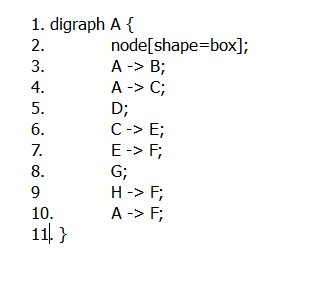
\includegraphics[width=\linewidth]{GV/gvcode.PNG}
        \caption{Simple graph}
        \label{figure : gv code}
    \end{subfigure}
    \begin{subfigure}[b]{0.4\linewidth}
    	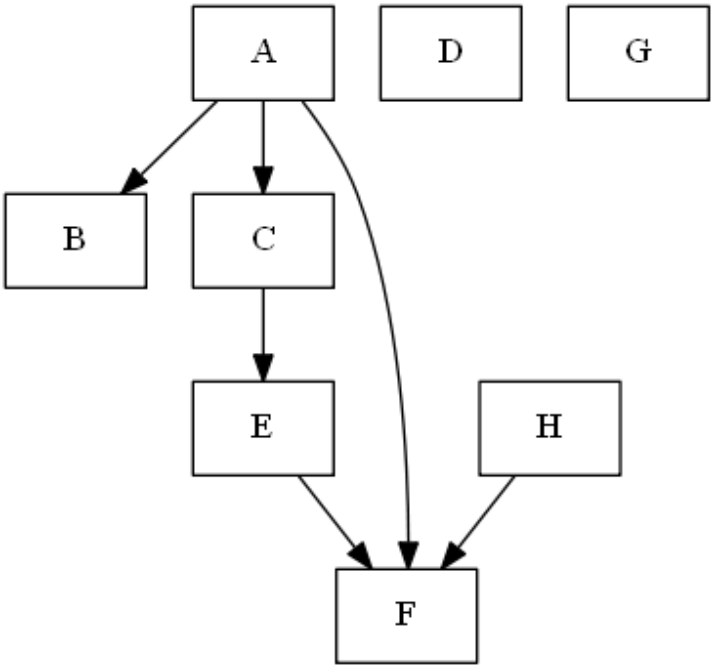
\includegraphics[width=\linewidth]{GV/gv1.PNG}
        \caption{Layout of simple graph}
        \label{figure : gv graph}
    \end{subfigure}
	\caption{Simple dot specification with layout}
    \label{figure : gv simple}
\end{figure}

\begin{figure}
	\centering
    \begin{subfigure}[b]{0.4\linewidth}
    	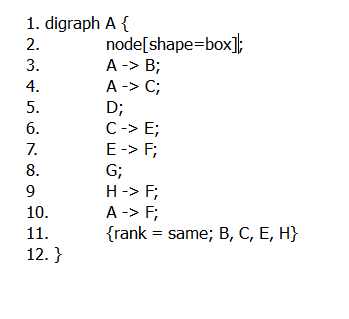
\includegraphics[width=\linewidth]{GV/gvcode_rank.PNG}
        \caption{Simple graph with \\ranking}
        \label{figure : gv rank}
    \end{subfigure}
    \begin{subfigure}[b]{0.4\linewidth}
    	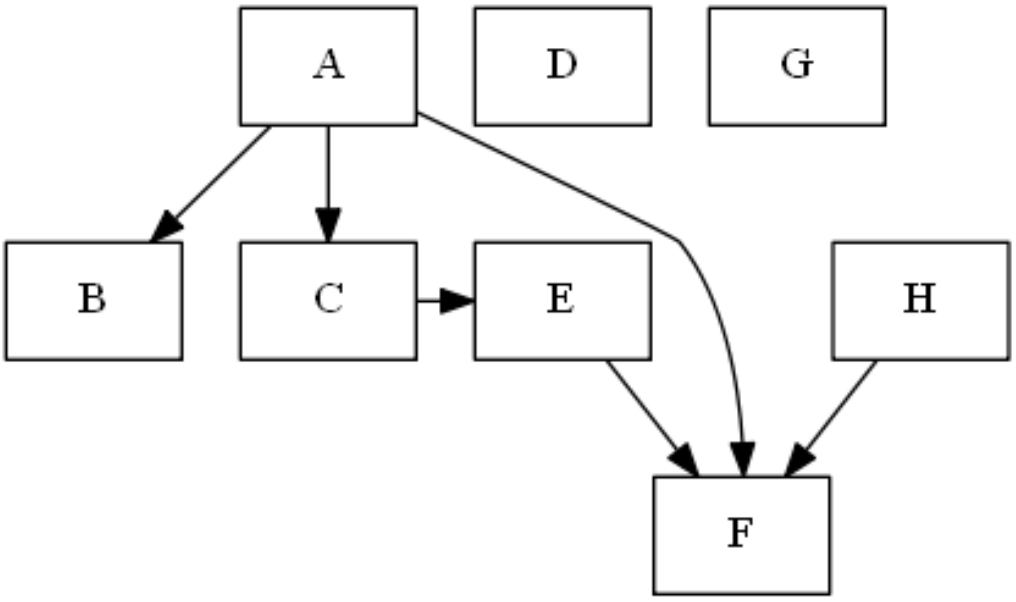
\includegraphics[width=\linewidth]{GV/gvrank.PNG}
        \caption{Layout of simple graph with ranking}
        \label{figure : gv graph rank}
    \end{subfigure}
	\caption{Dot specification and layout with ranking}
    \label{figure : gv with ranks}
\end{figure}

Figure \ref{figure : gv simple} illustrates a graph layout using GraphViz and the dot syntax.  Line 1 defines name and type of the graph while line 2 sets the shape of the node to box (see Figure \ref{figure : gv code}). The following lines, 3 to 10, create nodes and edges and link them accordingly (e.g., A -> B). The visual representation of this graph is shown in Figure \ref{figure : gv graph}. An example of a ranking constraint in a dot specification is depicted in Figure \ref{figure : gv with ranks}. Line 11 specifies a rank for nodes B, C, E, and H. This constraint forces the nodes to be at the same vertical or horizontal level. The default dot specification format is top-to-down drawing and thus the nodes have been constrained within a particular value of the y-coordinate. Close scrutiny of nodes C and E in Figure \ref{figure : gv with ranks} reveals that C is drawn first before E, from left to right. This is because, the source of the connecting edge is C while the target is E and dot tries to position source node left of target node in the same rank.

\subsection{mxGraph} \label{mxgraph}
 mxGraph is a graph library which enables users to quickly create graphs used for analysis, visualization, interaction, and layout \cite{JgraphX}. JGraphX is one of the graph library technologies embodied in mxGraph. mxGraph can be run in a web browser with a backend server or locally within a machine. The java library JGraphX of mxGraph is suitable for desktop applications while the Javascript implementation of mxGraph is preferred for web application \cite{JgraphX}. This section focuses on JGraphX, because it is the one currently used by TouchCORE. 
 
The layout algorithm of JGraphX assists users in a meaningful display of graph elements while avoiding overlap among the graph elements. The design model of JGraphX is shown in Figure \ref{fig : JGraphX Model}. The design model describes the structure and behaviour of JGraphX elements. mxGraphModel contains several operations used for adding, removing, and manipulating diagram elements. mxCell represents any element of the diagram such as an egde or node. mxGeometry specifies the layout information of each cell which includes the x, y, width, and height values. 

An example JGraphX snippet using hierarchical layout \cite{hierarchical_drawing} is shown in Figure \ref{fig : graphx samlpe code}.  After creating a new layout and setting the padding, the edges of the graph are set and the layout mechanism is executed. Finally, the model is updated to reflect the layout information. JGraphX supports various tree, force-directed, and hierarchical layouts \cite{JgraphX}.
 
\begin{figure}
	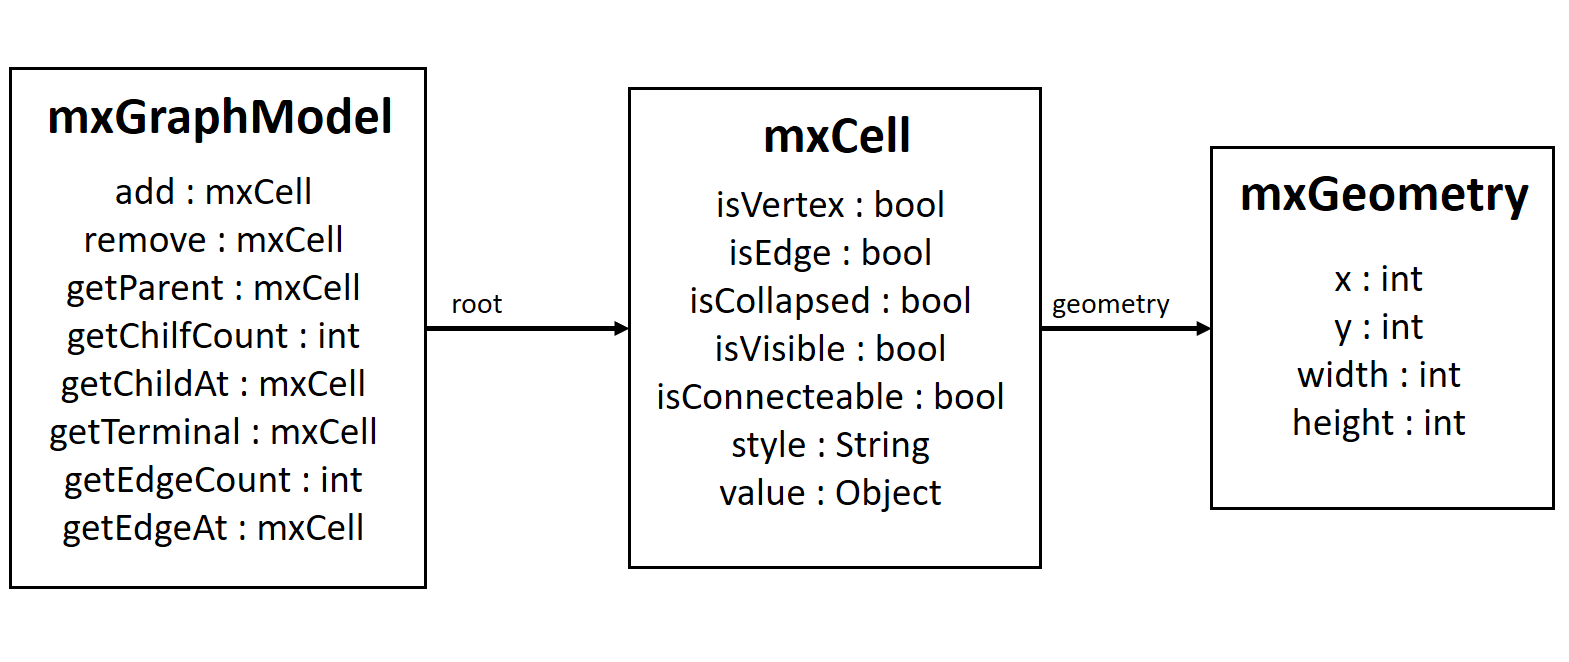
\includegraphics[width=\linewidth]{mxGraph.PNG}
	\caption{JGraphX design model \cite{mxGraph}}
	\label{fig : JGraphX Model}
\end{figure}

\begin{figure}
	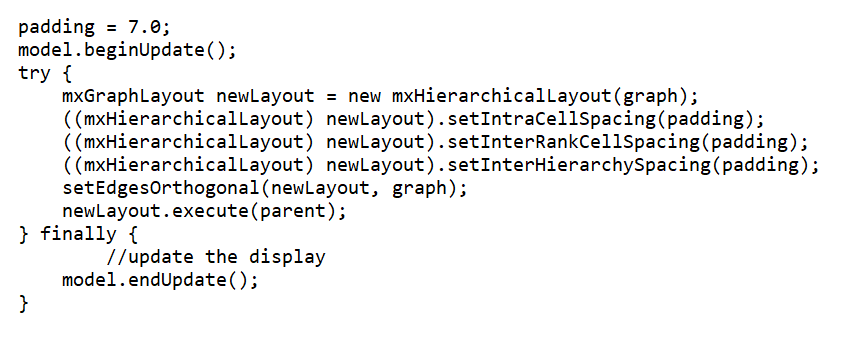
\includegraphics[width=\linewidth]{jgraphx.PNG}
	\caption{JGraphX sample specification}
	\label{fig : graphx samlpe code}
\end{figure}

\subsection{Other Layout Mechanisms} \label{RW}
This section discusses related layout mechanisms as identified by a search of the publications at the MODELS conference series and Google Scholar (see footnote \ref{f1}). 

Balazs \textit{et al.} \cite{gregorics2015textual} presents a \textit{textual diagram layout language} that allows modelers to describe the arrangement of model elements. The storing, editing, and versioning of models are better implemented in a textual language while graphical representation remains a preferred option for better comprehension. Balazs \textit{et al.} do recognize that automatic layout mechanisms often invalidate some intents of the modeler by arbitrarily rearranging model elements. To this end, the \textit{textual diagram layout language} is used to provide a concise layout description. Its basic idea is to define the position of nodes relative to others, e.g., \textit{Above(Box1, Box2)} means that Box1 is above Box2. While the basic idea of relative positioning is similar to rpGraph, the \textit{textual diagram layout language} does not address the layout of merged models during reuse. Furthermore, rpGraph infers the relative positioning of model elements from the existing layout while the \textit{textual diagram layout language} requires modelers to explicitly specify the layout  with the language.

\haAction{Keith Phalp \textit{et al.} presents a mechanism that merges layout diagrams by leveraging modelers to specify the order of classes and resolve conflict manually \cite{phalp2012supporting}. While this work endeavors to retain the meaningful layout of models after merge, similar to rpGraph, it uses the hierarchical information of the model elements unlike rpGgraph which considers the overall positioning of the elements. In addition, conflicts are automatically resolved in rpGraph while modelers resolve conflicts manually in their work. Merging is this work is like updating a layout, technically working on the same model diagram}


\haAction{
Yanling and Amber \cite{jin2012design} presents a Report Language Merging (RLM) aims to to keep the mental map of a model diagram undergoing several revisions. This work specifically targets the collaboration environment, where different individuals work on the same model and intend to merge their changes. They argue that much attention has not be given to merging of layout instead textual representation. Their work compares different versions of a model and present the outcome to user who manually make selection to avert some conflict if any exist. Colors are used to indicate the status of objects including deleted, inserted or changed. Inasmuch as this work uses color to assist in understanding changes in a model diagram, it does not address any relative positioning issues. In addition, it is semi-automated process, most of the activities are done manually unlike rpGraph.}

\haAction{
Jendrik and Karsten presents a generic layout composition framework which aims to preserve the mental map \cite{von2007mental} of model layouts after merging. The layout of merged model is based on a composition script specified by a modeler which dictates where model elements of each input diagram will be positioned. Comparing this work to rpGraph, the elements of each input diagram are bound together and configured manually where to be placed while rpGraph automatically infers the positioning of input diagram elements and adjust each element to maintain the original layout information after merging. Technically, the mechanism cannot handle any conflict such as cross-cutting of mapping elements which is handled automatically by rpGraph. 
}

Yosser and Cedric \cite{enhancingcommunication} argue that UML's graphical layout needs to be improved in order to enhance the communication among stakeholders. The color, orientation, and position of model elements, among others such as size, brightness, and grain/texture, are used to enhance  UML models as a vehicle of communication. Although, this work does not address relative positioning and layout of merged models during reuse, its aim, similar to rpGraph, is to retain the mental map of the stakeholders about the models. 
\haAction{
Similarly, Carsten \textit{et al.} presents \textit{GoVisual Approach} which aims to minimize bends, and crossing of edges, in addition to maintaining the hierarchy of a classes in a diagram \cite{gutwenger2003new}. Their algorithm takes a class diagram and rearranges the classes such that super classes are always above the subclass while the number of crossing is  minimized. The work further adds colour to a particular generalization in the class diagram for easy recognition of family of classes. While this work aims to enhance the visualization and understanding of a layout, the mechanism rearranges the layout in a specific format that could distort the mental map of the model. Unlike rpGraph, the mechanism only works on single class diagram and fail to address merging of two or more diagrams. 
}

 Evolution of software is spread across all software artifacts. Therefore, when a graphical modeling language is updated, migrating existing models may lead to improper layout such as overlap of nodes. Ult \textit{et al.} \cite{incrementaldiagram} presents a layout algorithm based on network simplex which rearranges the model elements to depict a proper layout\haAction{, i.e., layout that retains the original positioning of model elements after update,} while keeping the general framework of the model. This model adjustment keeps models synchronized with changes to software tools and language. However, the layout of a merged model during reuse is not addressed. 
\haAction{
In a similar  way, Sonja and Mark present mechanism to record, process, and visualize diagram changes \cite{maier2015recording}. The algorithm records the snap-shop of changes including delete, add, move, or create nodes in a diagram. While this approach aids in keeping a concise and comprehensive view of diagrams after changes, it does not address the visualization of merged layout diagrams. Moreover, rpGraph infers the positioning of layout nodes from the diagram unlike these algorithms that keep track of changes done by the users.
}

\section{rpGraph Layout Algorithm}\label{The work}
As a possible solution to the challenges of determining a proper layout of merged model elements, this work proposes an algorithm to retain the original layout information while avoiding edges and elements overlap. The algorithm operates on the proposed rpGraph metamodel which establishes relative relationships among model elements. This section details the metamodel first and then explains how we intend to use it to solve the problem of proper layout of merged models after reuse.

\subsection{Layout Metamodel of rpGraph} \label{metamodel section}
This section describes the abstract syntax and semantics of our metamodel shown in Figure \ref{fig : metamodel diagram}. The LayoutModel contains a set of Nodes and a set of Edges, with each Edge going from a source Node to a target Node. The position relationships covered by Edge in the metamodel are Above, DirectAbove, Left, and DirectLeft. The Above relationship exists between two Nodes (i.e., rectangles) where the source Node is above the target Node when visualized. The same relationship applies to Left: the source Node should be at the left of the target Node when visualized. Additionally, DirectAbove is when the source Node is \haDeleted{fairly} directly above the target Node, i.e., a vertical line extending the left or right side of the source Node touches the target Node. \haAction{As shown in Figure \ref{fig :Bank App}, Session is directly above Password, however, Session is above |ProtectedClass and not directly above it.} Similarly, a horizontal line extending the top or bottom sides of the source Node touches the target Node in the case of DirectLeft. These relationships are intended to be used while visualizing the model to make sure that their relative positions are maintained, and overlaps of nodes and edges are minimized. The following points highlight additional features of the relationships.

\begin{itemize}
\item \textbf{Above:} An Above relationship is established for all Nodes below a Node. If Node A is above Node B which is above Node C, then three relationships are created: A above B, A above C, and B above C. This approach is preferred over an approach that exploits transitivity, because it simplifies processing of the LayoutModel later on.
\item \textbf{DirectAbove:} In some cases, a target Node that is directly below the source Node behaves differently when visualized \haReplace{because there is no Left relationship between the two Nodes. The target may hence be placed freely left or right of the source Node.}{especially when it does not have source Node based on Left or DirectLeft relationship. The target Node may hence be placed freely far left of the above source Node especially when the target node is from a model that needs to be positioned right of another model after merging.} To solve this problem, we introduced DirectAbove as shown in Figure \ref{fig : metamodel diagram}. \haAction{This relationship ensures that the target node is restrained from moving left of the source above node.}
\item \textbf{Left:} Similar to Above, a Left relationship is established for all Nodes right of a Node (if Node A is left of Node B which is left of Node C, then three relationships are created: A left of B, A left of C, and B left of C). 
\item \textbf{DirectLeft:} Similar to DirectAbove, we use DirectLeft to restrain Nodes from being positioned freely above the source Node even though it should be situated right next to the source Node.
\end{itemize}

\begin{figure}
	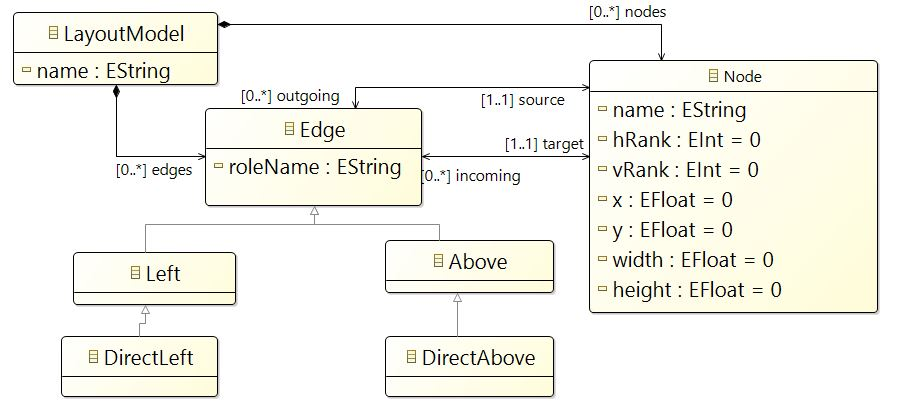
\includegraphics[width=1\linewidth]{metamodel}
	\caption{Layout metamodel}
	\label{fig : metamodel diagram}
\end{figure}

\subsection{The rpGraph Layout Algorithm}\label{rpGraph algorithm}
This section describes the rpGraph layout algorithm of a merged model. This algorithm is based on the metamodel (see Section \ref{metamodel section}), employs GraphViz (see Section \ref{graphviz}) as the backend, and is implemented in the TouchCORE tool (see Section \ref{touchcore}). The following subsections detail the algorithm while an overview of the algorithm is shown in Figure \ref{fig :main algorithm}.

\begin{figure}
	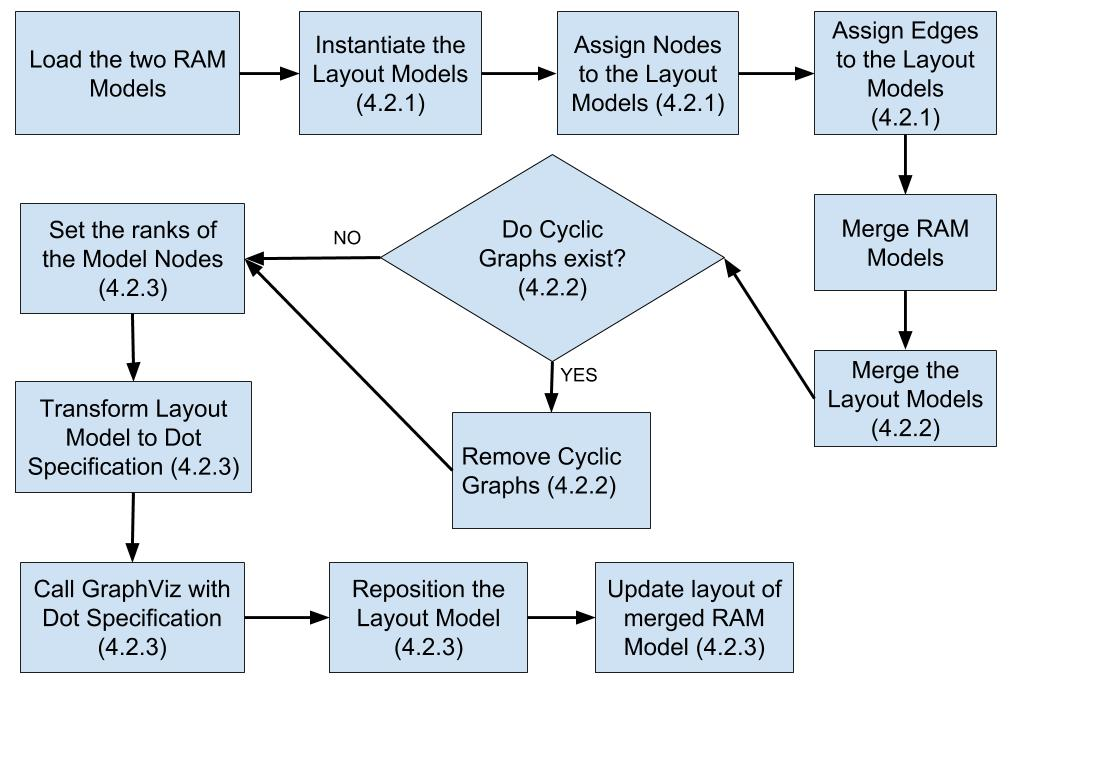
\includegraphics[width=1\linewidth]{LayoutFlow.jpg}
	\caption{rpGraph algorithm}
	\label{fig :main algorithm}
\end{figure}

\subsubsection{Create layout models} \label{create layout model}
The RAM models of the reused and reusing models are maintained by the TouchCORE tool. The x-coordinate, y-coordinate, width, and height values of each model element are used as parameters to instantiate the Node class in the metamodel (see Figure \ref{fig : metamodel diagram}). Prior to creating instances of Node, two LayoutModels are instantiated, one corresponding to the reusing (higher) model and one to the reused (lower) model. Following these instantiations, each Node instance is added to its corresponding LayoutModel instance.

Afterwards, we create and assign Edge instances to nodes based on their attributes. At this juncture, we evaluate each node using its x-coordinate, y-coordinate, width, and height to establish its position with respect to all other nodes in the model. The evaluation of relative positions of each element is based on its original model. Exactly one DirectAbove relationship, or exactly one DirectLeft relationship, or exactly one pair of Above and Left relationships is created for each pair of two nodes in a model.

\subsubsection{Merge layout models}
Having transformed the two models to layout models, we merge the two using the weaving information \cite{alam2013concern} provided by TouchCORE, i.e., after TouchCORE has merged the two RAM models (see Figure \ref{fig :main algorithm}). During the layout merging, each mapped element from the lower model, i.e., the reused model, is removed while its edges are copied into the corresponding higher mapped element\haAction{, i.e., the reusing model elements.} The result of this merge can lead to a cyclic graph because of the assigned edges of the nodes.
\begin{figure}
	\centering
    \begin{subfigure}[b]{0.4\linewidth}
    	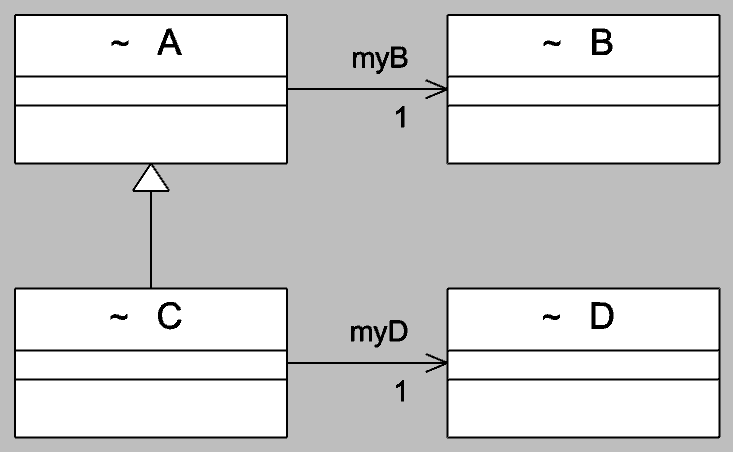
\includegraphics[width=\linewidth]{cyclicm1.PNG}
        \caption{Reusing model}
        \label{figure : cyclic1}
    \end{subfigure}
    \begin{subfigure}[b]{0.4\linewidth}
    	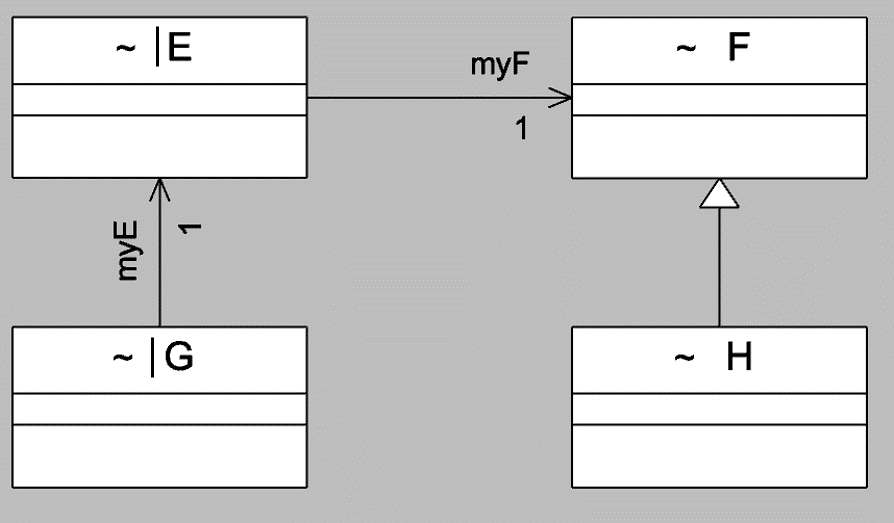
\includegraphics[width=\linewidth]{cycllic2_update.png}
        \caption{Reused model}
        \label{figure : cyclic2}
    \end{subfigure}
	\caption{Cyclic graphs}
    \label{figure : cyclicgraph}
\end{figure}
\haReplace{For example, a lower element E may be mapped to a higher element D and another lower element G may be mapped to higher element B and E is above G while B is above D as shown in Figure \ref{figure : cyclicgraph}. }{For example, a lower element E may be mapped to a higher element D and another lower element G may be mapped to higher element B. In reused model, E is above G while B is above D in the reusing model as shown in Figure \ref{figure : cyclicgraph}. }During the edge assignment, an Above edge is assigned to E and G, where E is the source and G is the target. Similarly, an Above edge is assigned to B and D, where B is the source and D is the target. However, due to the merging of the two layout models, class E and D have been combined into one class D, and class G and B have equally been combined into one class B. This implies that B has two above relationships where D is the source element in one and target element in the other. This leads to a cyclic graph. In order \haAction{to avoid infinite runtime during ranking of model elements,} \haAction{i.e., the iteration to get nodes above D will return B, which will in turn return D as a node being above B and so on ...,} \haDeleted{apply GraphViz (which does not support cyclic graphs) as the backend of the rpGraph layout algorithm,} we therefore remove the relationship \haReplace{belonging to the lower model (the reused model)}{established between E and G.} Because, we give higher priority to the higher model (the reusing model) as the lower model is merged into it. The next section explains how we use GraphViz to reposition the layout model elements based on relative position information.

\subsubsection{Reposition the layout with GraphViz}
Having created the merged layout model with its nodes and edges (Above, DirectAbove, Left, and DirectLeft), we aim to use the attributes of the layout model to reposition its nodes accordingly. 

In the first place, prior to the transformation of the model to dot specification, we assign ranks to each model element as shown in the attributes of the Node class in the metamodel (see vRank and hRank in Figure \ref{fig : metamodel diagram}). We assign two ranks per element, vertical and horizontal ranks. Vertical ranking is top-down while horizontal ranking is left-right starting from number one. We use the edges of a node to determine its rank recursively. \haAction{The pseudo-code of the ranking algorithm is shown in Figure \ref{fig :ranking}. The diagram shows how vertical ranks are determined which is similar to horizontal ranks except that Left, and DirectLeft edges are used for horizontal ranking. The algorithm first checks if the node has any incoming edge (Above or DirectAbove), else the vertical rank is 1. e.g., the rank of node A in Figure \ref{fig :model ranks} is 1, (lines 3-5 in Figure \ref{fig :ranking}). However, if there is incoming Above or DirectAbove,  there are above nodes and they are stored as a list of nodes, (lines 7-13 in Figure \ref{fig :ranking}). Each node in the list is processed to determine its rank by calculating the highest number of nodes above it using recursive technique, (lines 14-23 in Figure \ref{fig :ranking}).} 

\begin{figure}
	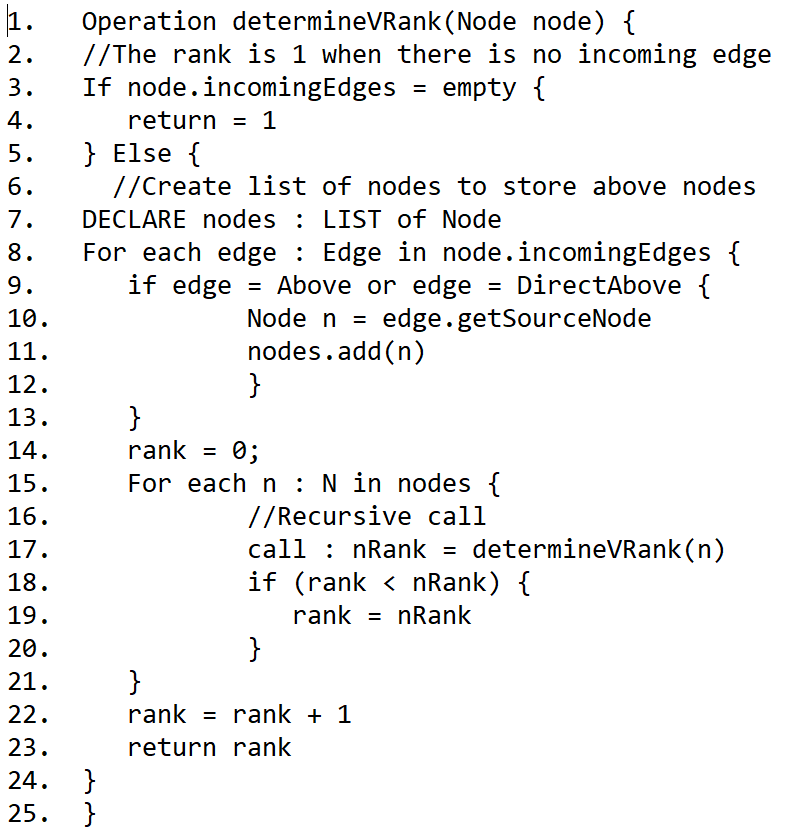
\includegraphics[width=\linewidth]{ranking.PNG}
	\caption{Nodes ranking}
	\label{fig :ranking}
\end{figure}
\begin{figure}
	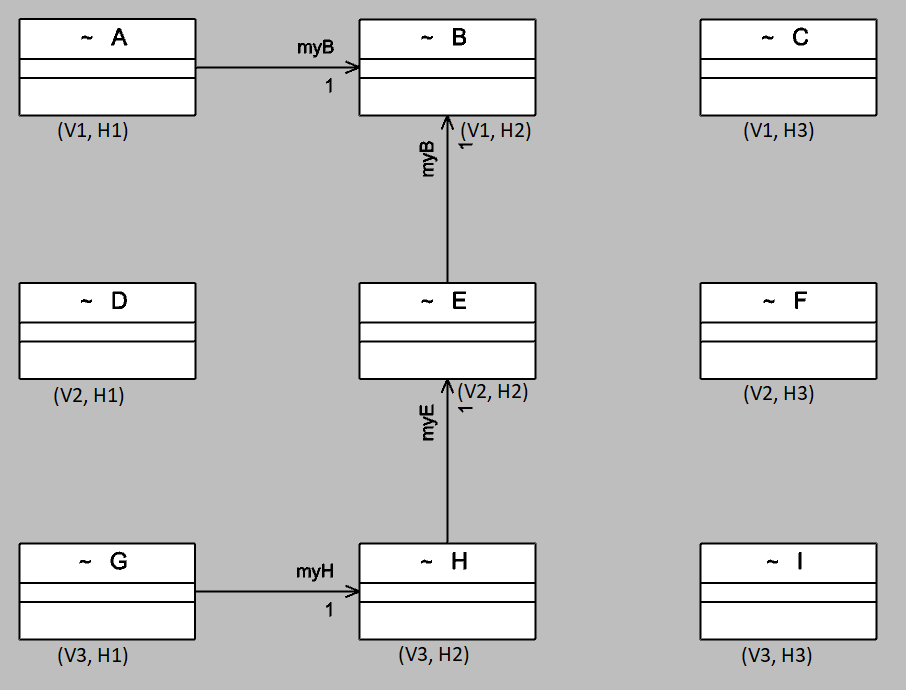
\includegraphics[width=1\linewidth]{sample_algorithm2.PNG}
	\caption{Ranking of nodes (vertical and horizontal ranks are indicated in parentheses next to a node)}
	\label{fig :model ranks}
\end{figure}
\begin{figure}
	\centering
    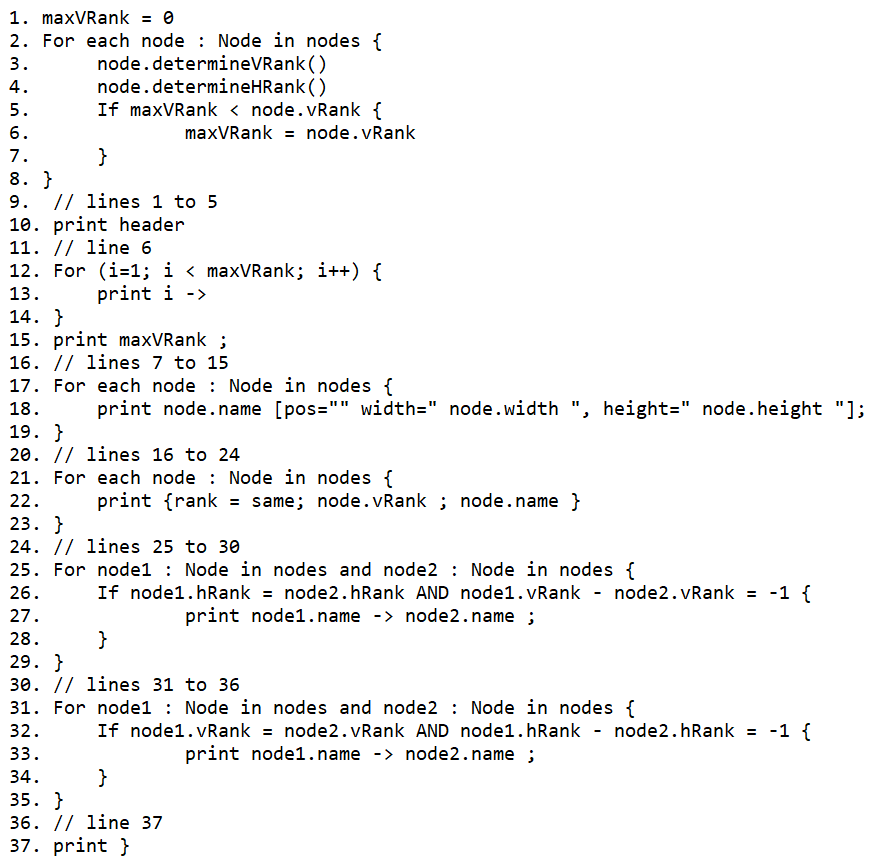
\includegraphics[width=\linewidth]{pseudocode.PNG}
    \caption{Layout model to dot transformation (the comments // include references to the lines in Figure \ref{fig : dot code})}
    \label{fig : pseudocode}
\end{figure}
\begin{figure}
	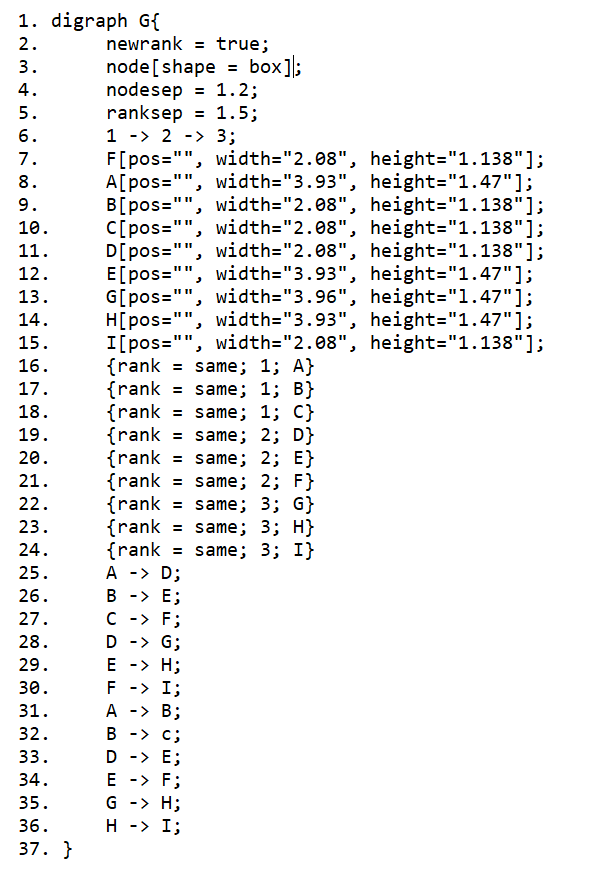
\includegraphics[width=0.7\linewidth]{dotcode.PNG}
	\caption{Dot specification of the sample model}
	\label{fig : dot code}
\end{figure}

Figure \ref{fig :model ranks} shows an annotated model to illustrate the ranking of nodes, V1 is vertical rank 1 and H1 is horizontal rank 1 and so on. As shown, node A is above node D and node D is above node G. It implies that node A, D, and G have a vertical rank of V1, V2, and V3, respectively. Similarly, node A is left of node B and node B is left of node C. This also implies that node A, B, and C have horizontal rank of H1, H2, and H3, respectively. The rpGraph layout algorithm sets the vertical ranks using Above and DirectAbove edges while Left and DirectLeft are used for the horizontal ranking (lines 3-4 in Figure \ref{fig : pseudocode}). These rank values are used in addition to other attributes of the nodes during the transformation to dot. As explained in Section \ref{graphviz}, nodes can be ranked vertically or horizontally in GraphViz but not both at the same time. In this work, we apply the vertical ranks to constrain a set of nodes within a distinct level (lines 1, 5-7, 11-15, and 20-23 in Figure \ref{fig : pseudocode}; lines 6 and 16-24 in Figure \ref{fig : dot code}). On the other hand, both the horizontal and vertical ranks are used during the connection of the nodes with the -> operator (lines 24-29 for vertical ranks and 30-35 for horizontal ranks in Figure \ref{fig : pseudocode}; lines 25-30 and lines 31-36, respectively, in Figure \ref{fig : dot code}). For example in Figure \ref{fig :model ranks}, the same vertical rank V1 ensures that A, B, and C are constrained within the first level. Horizontal ranks are used to position the nodes within a vertical rank. Since node A is left of node B while A and B are on the same vertical rank, the corresponding dot specification is A -> B. This approach is applied to all nodes to obtain the corresponding specification in the dot notation. Figure \ref{fig : dot code} shows the corresponding dot specification for Figure \ref{fig :model ranks}. The resulting dot specification is fed to GraphViz to obtain the new x and y coordinates of each node. The new coordinates are consequently used to update the merged model accordingly.

\haAction{
\subsection{GraphViz Layout Algorithm}
In this work, the layout models of rpGraph are compared against the layouts of GraphViz using dot language. Hence, we present in this section the steps followed to produce the GraphViz layout models as shown in Figure \ref{fig : gv algorithm}. First, we create node in dot notation for each RAM model element and initialize its attributes using the width and height of the corresponding RAM element ( lines 1-3 in Figure \ref{fig : gv algorithm}). These nodes are created arbitrarily as TouchCORE tool does not iterate over the model elements using any specific order. Each association of the model elements maintained by TouchCORE tool is used to create a corresponding link in the dot specification, (lines 4-6 in Figure \ref{fig : gv algorithm}), where the source node represents the source of the association, and the target node represents the target of the association. For generalization, a dot link is created for each inheritance, the source node of the link represents the super class while the target node stand for the sub class. The GraphViz algorithm used in this work is top-down and thus, we aim to draw the super class node above subclass node. Generally, we aim to produce a dot specification structurally similar to the input RAM models. The next step is to feed the dot specification (see Figure \ref{gv dot}) to GraphViz back-end which produces new x and y coordinates of each node which are used to update the RAM model elements accordingly.
 }
\begin{figure}
	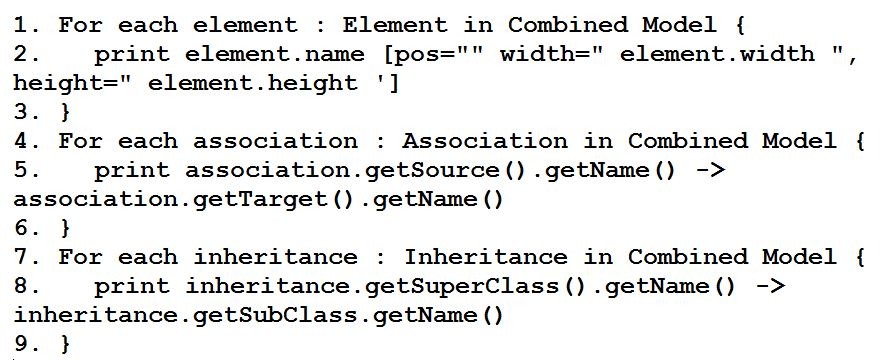
\includegraphics[width=1\linewidth]{gvAlgorithm}
	\caption{Pseudocode of GraphViz layout algorithm }
	\label{fig : gv algorithm}
\end{figure}
 
\begin{figure}
	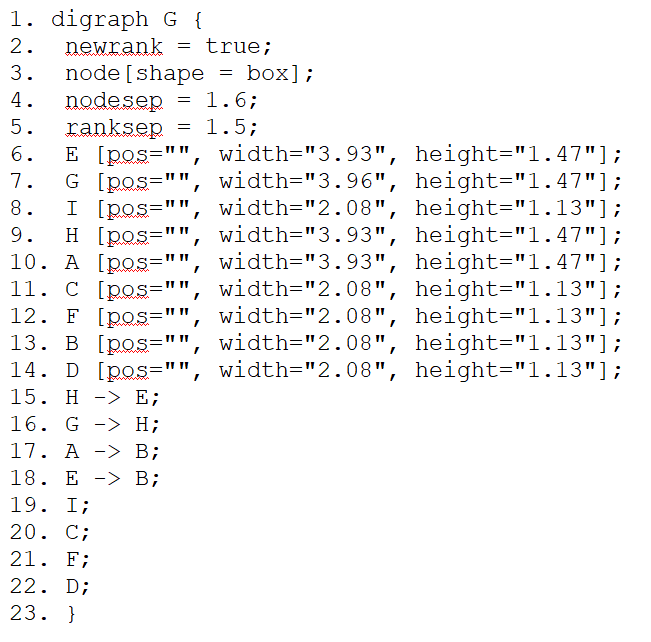
\includegraphics[width=1\linewidth]{gvDot.PNG}
	\caption{GraphViz dot specification }
	\label{gv dot}
\end{figure}
\subsection{Examples}
In this section, we illustrate the layout problem with two examples, show how our algorithm stands to address the issue, and visually compare our results with related layout solutions, i.e., the de-facto layout standard GraphViz and JGraphX, which is the layout mechanism currently used in the TouchCORE tool. Figure \ref{figure : sample} depicts two models with the desired layout. Model 1 reuses Model 2 with class M in Model 2 being mapped to class F in Model 1, i.e., M and F are combined in the merged result.

\begin{figure}
	\centering
    \begin{subfigure}[b]{.4\linewidth}
    	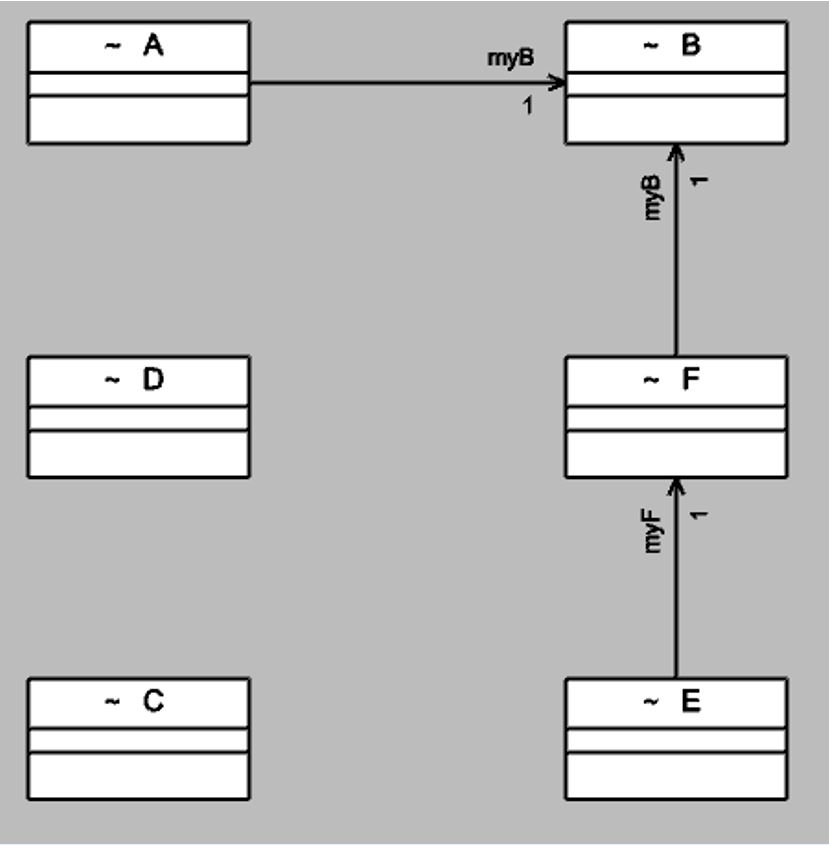
\includegraphics[width=\linewidth]{reuse1}
        \caption{Model 1}
    \end{subfigure}
    \begin{subfigure}[b]{.4\linewidth}
    	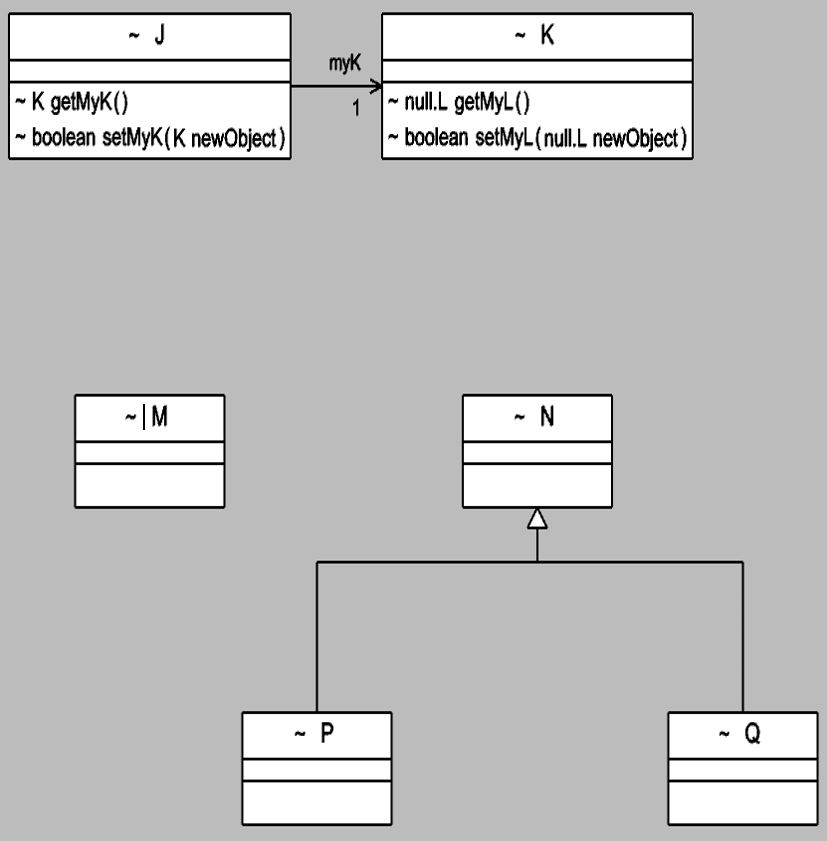
\includegraphics[width=\linewidth]{reuse2}
        \caption{Model 2}
    \end{subfigure}
	\caption{Reuse maps M in model 2 to F in model 1}
    \label{figure : sample}
\end{figure}

\begin{figure}
	\centering
    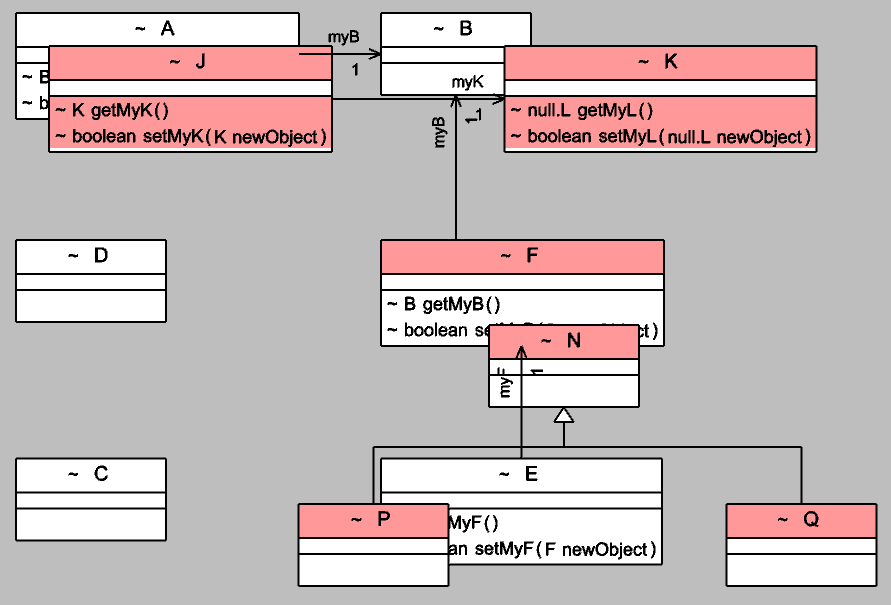
\includegraphics[width=1\linewidth]{default_sample.PNG}
    \caption{Default merged model}
    \label{fig : default sample}
\end{figure}

\begin{figure*}
	\centering
    \begin{subfigure}[b]{1\linewidth}
    	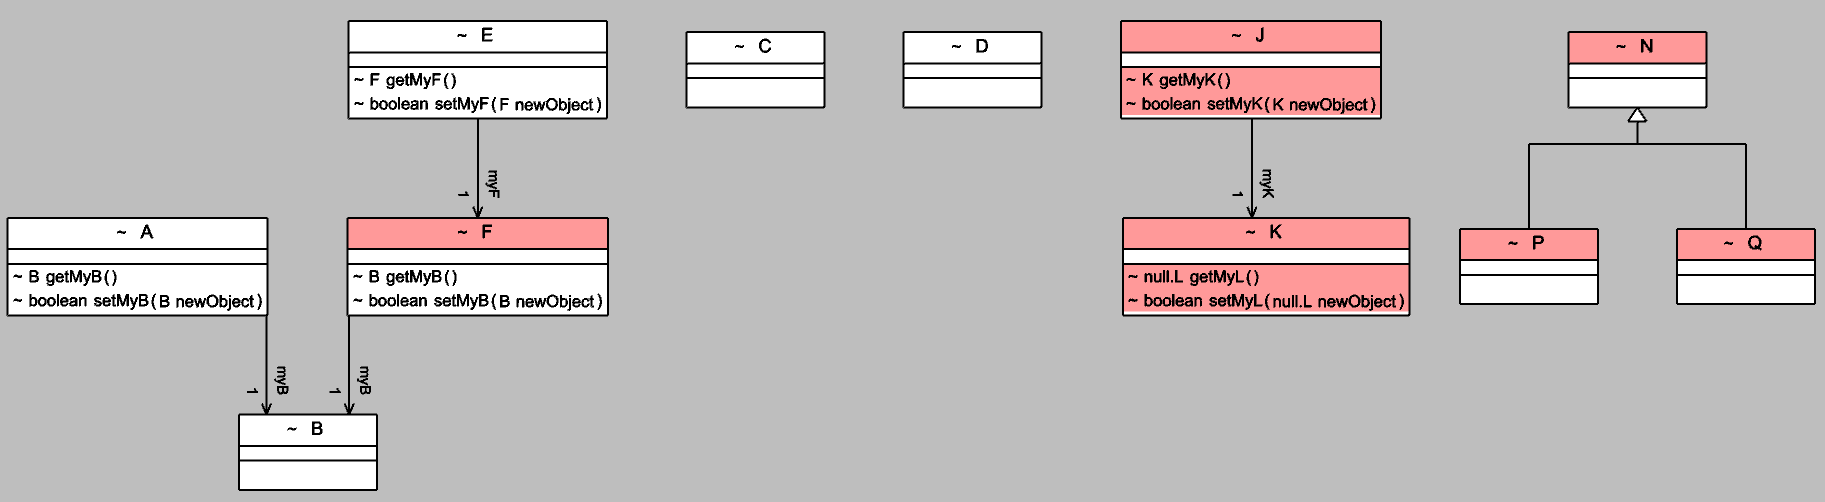
\includegraphics[width=\linewidth]{gv_sample.PNG}
        \caption{GraphViz}
        \label{figure : gv sample}
    \end{subfigure}
    \begin{subfigure}[b]{1\linewidth}
    	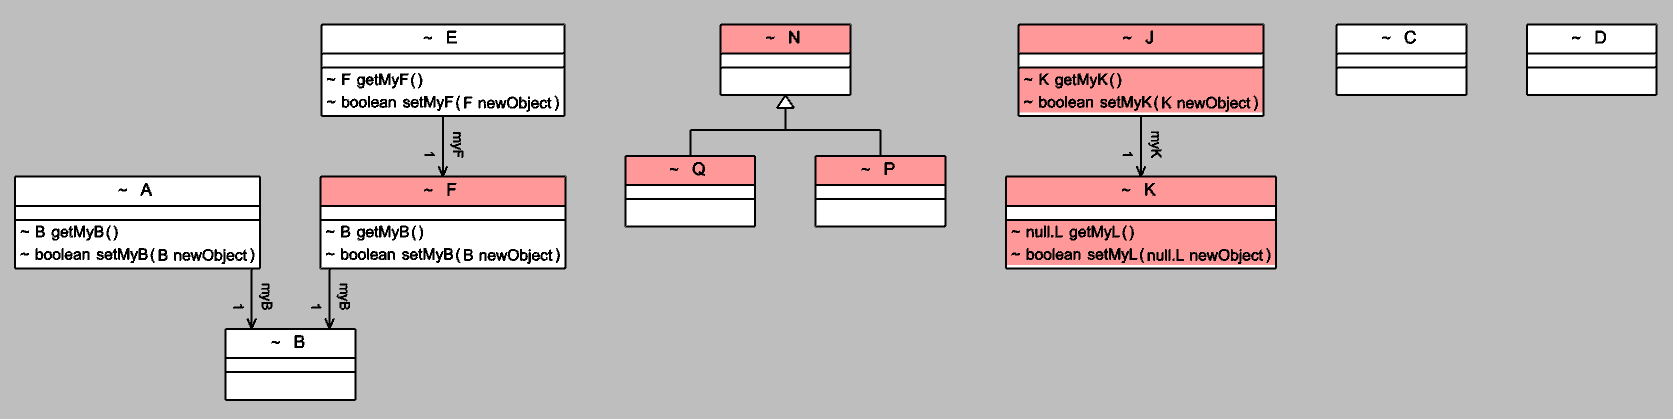
\includegraphics[width=\linewidth]{gx_sample.PNG}
        \caption{JGraphX}
        \label{figure : gx sample}
    \end{subfigure}
    \begin{subfigure}[b]{1\linewidth}
    	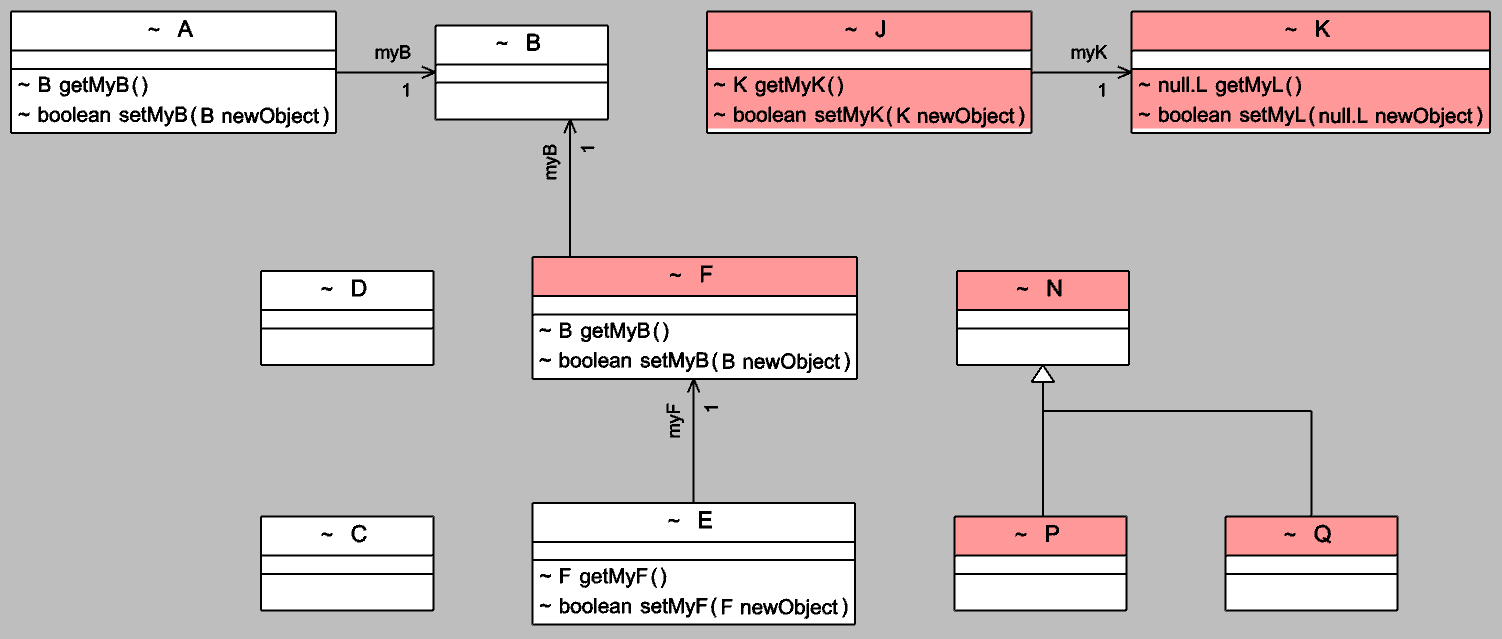
\includegraphics[width=\linewidth]{rp_sample.PNG}
        \caption{Relative positioning (rpGrah)}
        \label{figure : rp sample}
    \end{subfigure}
	\caption{Comparison of layout solutions of merged model 1 and model 2}
    \label{figure : sample solution}
\end{figure*}

When these models are merged together without the application of any automatic layout algorithm, the model elements overlap one another as they retain their original positions as shown in Figure \ref{fig : default sample}. The result of the automatic layout approaches GraphViz, JGraphX (TouchCORE), and rpGraph are depicted in Figure \ref{figure : sample solution}  with the reused model highlighted in pink color and the reusing model shown with white background. Close inspection of the models in Figure \ref{figure : sample solution} reveals that rpGraph maintains the relative location of model elements of each model while keeping the model dimension ratio fairly constant and avoiding additional free space in the merged model. On the other hand, the GraphViz and JGraphX solutions reorder the model elements arbitrarily which leads to loss of important information conveyed by the original model layout. \haAction{For example, the original reuse model shows that B is above F while F is above E but this ordering is reversed in the merged model using GraphViz or JGraphX. Another important loss of information is the placement of B under A instead of right of A, as shown in the merged model of GraphViz or JGraphX.} As another example, consider the authentication and bank application models from Figure \ref{fig :Authentication Concern} and Figure \ref{fig :Bank App}, respectively, as well as the default merged layout shown in Figure \ref{fig : default bank and authentication}. |Authenticatable and |ProtectedClass in authentication are mapped to User and AccountManager in \haAction{the} bank application, respectively. The results of the automatic layouts of GraphViz, JGraphX (TouchCORE), and rpGraph are shown in Figure \ref{figure : bank solution}. \haReplace{and similar observations can be deduced from the models.}{Similarly, rpGraph keeps the original relative positioning of the model elements while GraphViz, and JGraphX reorder the layout to the extent that most of the original relative positioning is lost. Examples, the layout mental map of the bank application is completely lost as the model elements of the reused or reusing model are scattered and interspersed with other model elements in the merged model of both JGgraphX and GraphViz.} 

In the next section, the three automatic layout algorithms are compared with each other more formally with the help of a set of metrics characterizing the layout of the reused model, the reusing model, and the merged result.

%\begin{figure}
%	\centering
 %   \begin{subfigure}[b]{0.4\linewidth}
  %  	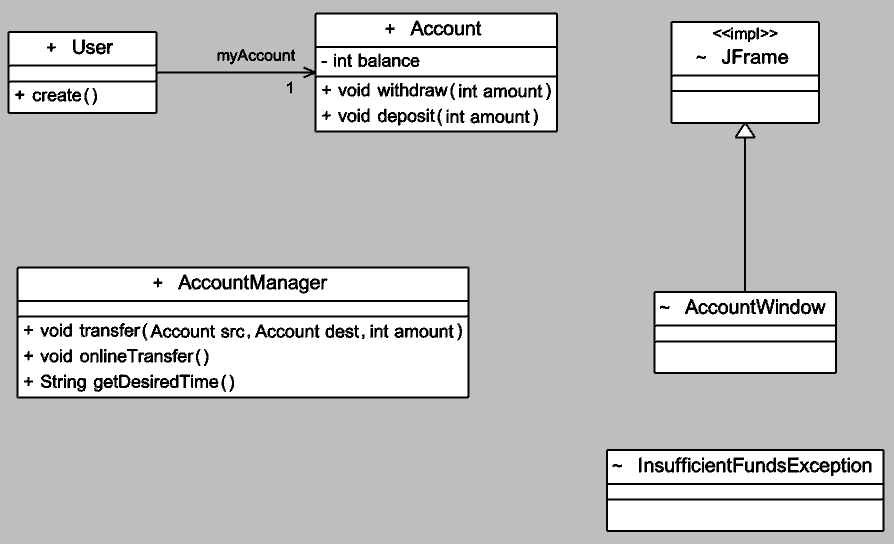
\includegraphics[width=\linewidth]{bank.PNG}
   %     \caption{Bank Application}
    %    \label{figure : bank}
    %\end{subfigure}
    %\begin{subfigure}[b]{0.4\linewidth}
    %	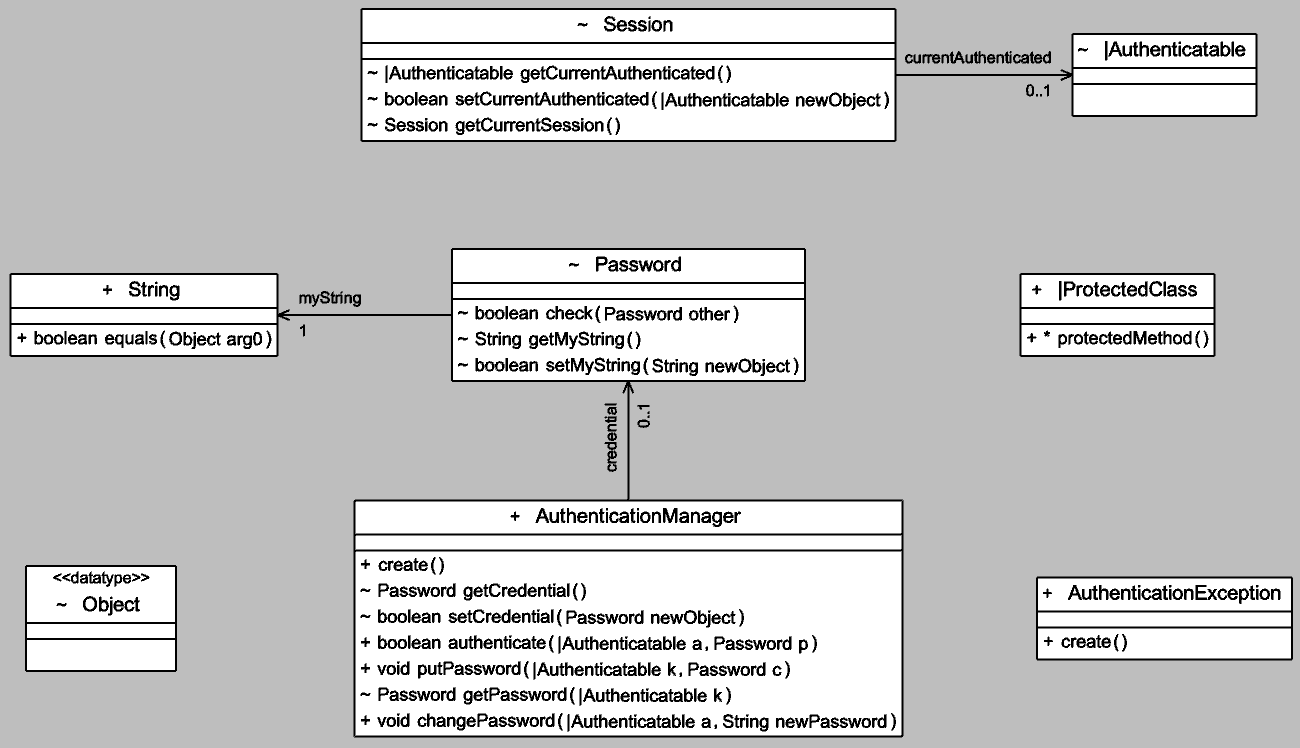
\includegraphics[width=\linewidth]{authentication.PNG}
     %   \caption{Password Authentication}
      %  \label{figure : Authentication}
    %\end{subfigure}
	%\caption{Bank Application reuses Password Authentication}
    %\label{figure : bank and authentication}
%\end{figure}

\begin{figure*}
	\centering
    \begin{subfigure}[b]{1\linewidth}
    	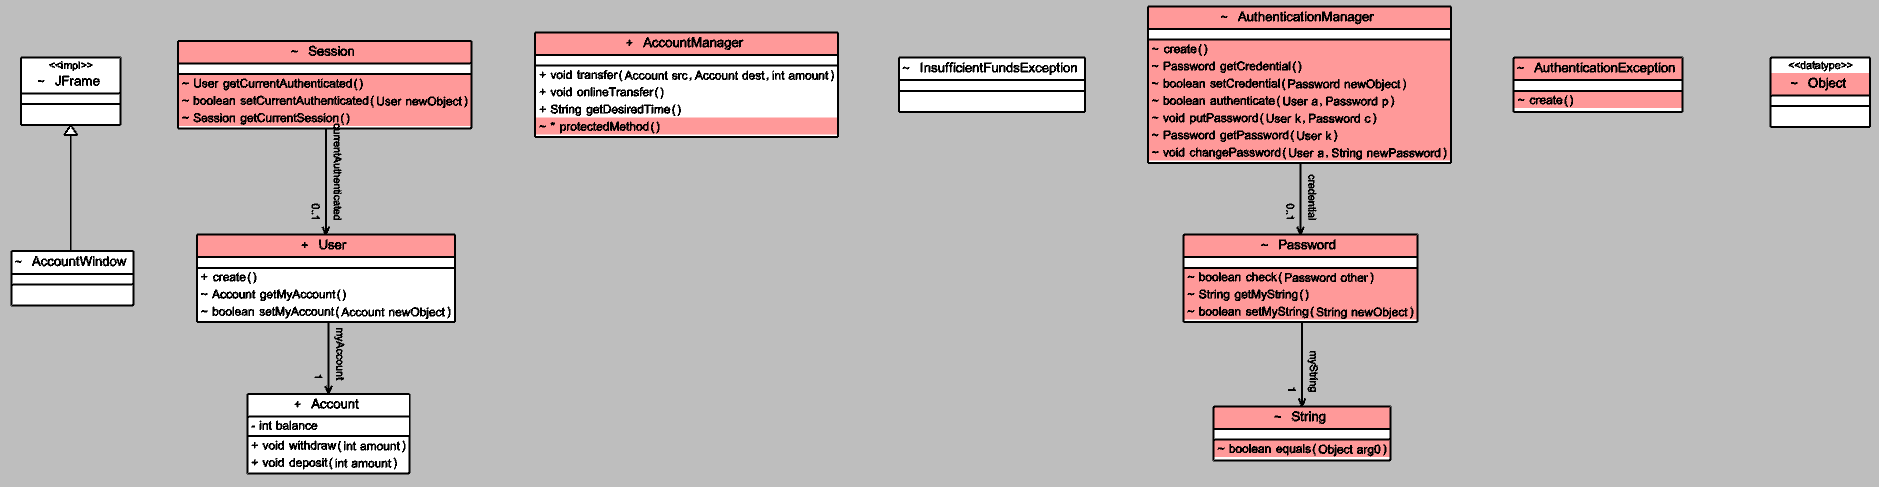
\includegraphics[width=\linewidth]{gv_bank.PNG}
        \caption{GraphViz}
        \label{figure : gv bank}
    \end{subfigure}
    \begin{subfigure}[b]{1\linewidth}
    	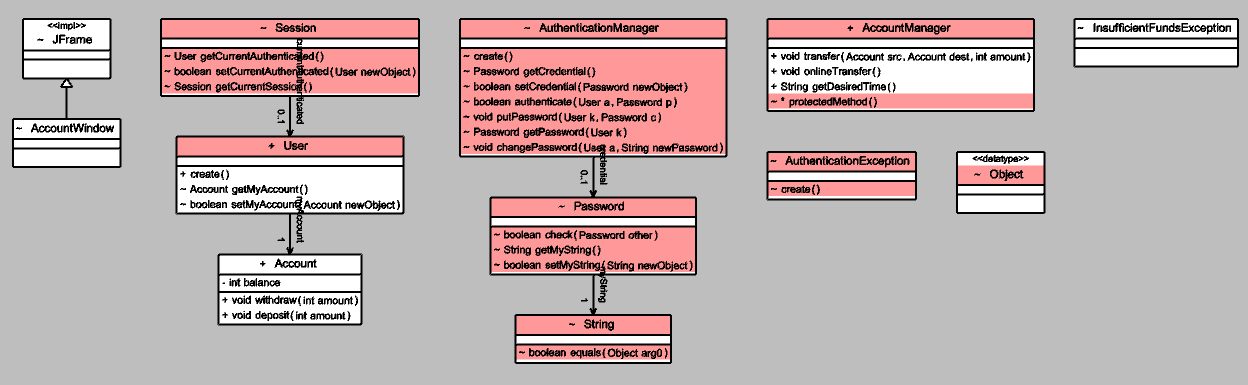
\includegraphics[width=\linewidth]{gx_bank.PNG}
        \caption{JGraphX}
        \label{figure : gx bank}
    \end{subfigure}
    \begin{subfigure}[b]{1\linewidth}
    	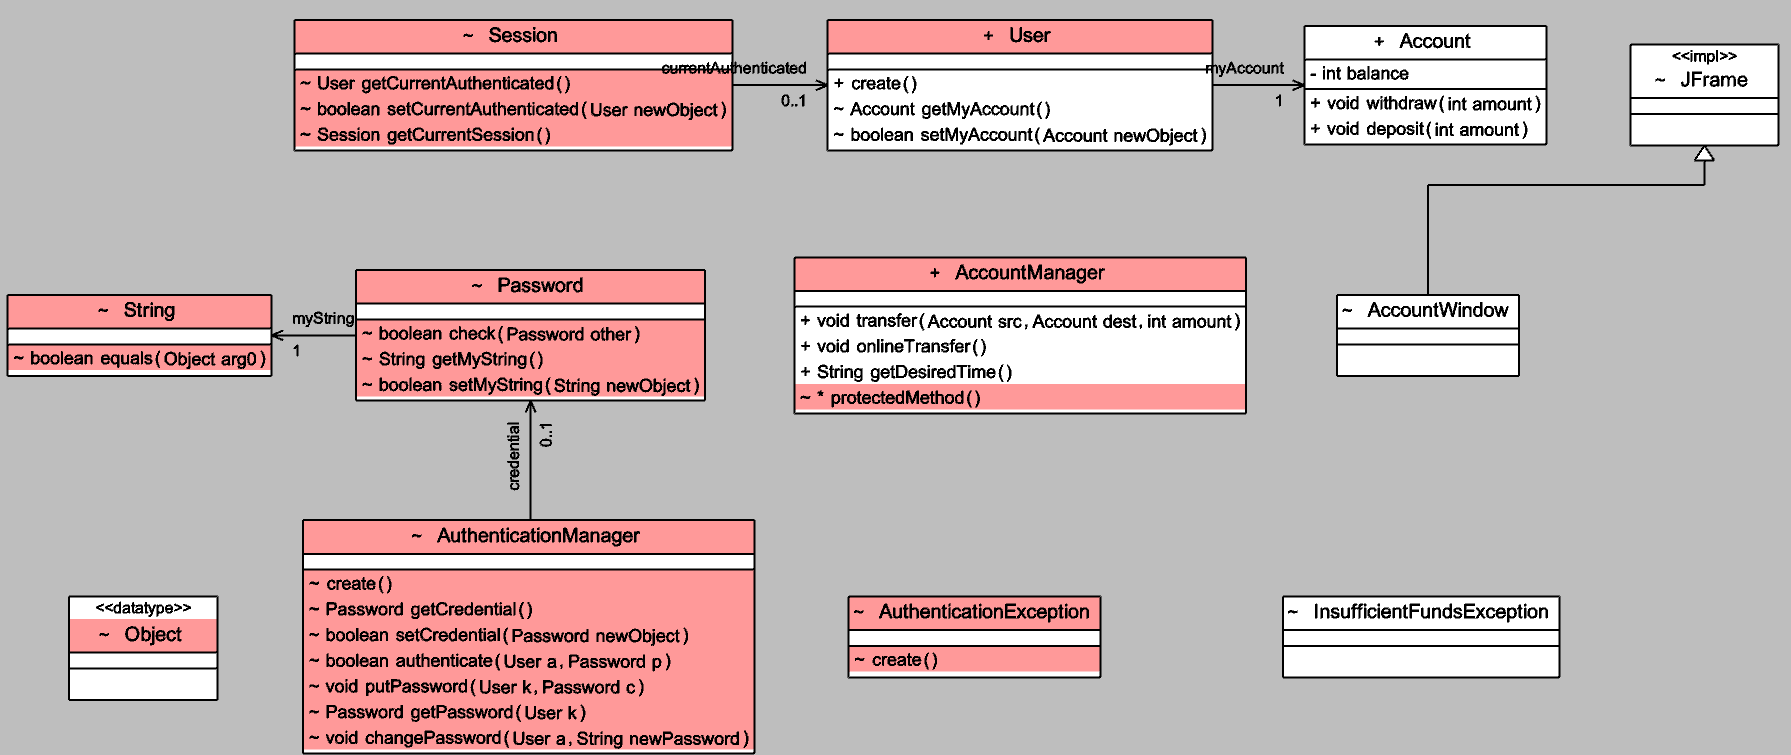
\includegraphics[width=\linewidth]{rp_bank.PNG}
        \caption{Relative positioning (rpGraph)}
        \label{figure : rp bank}
    \end{subfigure}
	\caption{Comparison of layout solutions of merged bank and authentication}
    \label{figure : bank solution}
\end{figure*}

\section{Results and Discussion}\label{discussion}
In this section, we \haAction{present the layout comparison metrics and} evaluate our rpGraph algorithm by comparing its layout of merged models with two notable layout algorithms, GraphViz (GV) and JGraphX (GX). In this evaluation, we denote our algorithm as Relative Positioning (RP). We use existing reusable RAM models (class diagrams) including authentication, access control, and workflow from the TouchCORE library of reusable models. In total, we selected 20 reusable artifacts and each is reused in a specific context such as bank, door, or accounting applications \haAction{(see Table \ref{table:1})}. The number of classes in each reusing model ranges from 2 to 17 while the reused models have between 1 to 20 classes each. The number of classes in each merged model spans from 2 to 35. The number of pairs of mapped classes used in the evaluation ranges from 1 to 4 for each model reuse. All the original and merged models used in this evaluation are available in the rpGraph GitHub repository\footnote{The individual and merged models, merged model of rpGraph, GraphViz, and JGraphX can be found in GitHub, https://github.com/Hyacinth-Ali/AutoLayoutDataset/tree/master/LayoutImages. Pink color elements are reused elements while white elements are reusing elements. The name of the models rx, gv, and gx correspond to the layout of rpGraph, GraphViz, and JGraphX, respectively.}. 

\haAction{
\begin{table}
\centering
\begin{tabular}{ |c|c| } 
\hline
\textbf{Reusing Model} & \textbf{Reused Model} \\
\hline
Bank & Authentication \\ 
Demo & Minueto \\ 
Door & Access Control \\ 
Workflow & Copyable \\
Input Output & Singleton \\
Input & Name \\
Input Output & Command \\
Conditional & Named \\
Command & Named \\
Inpath & Named \\
Checkpoint & Copyable \\
Traceable & Access \\
Accounting & Authentication \\
Accounting & Mortgage \\
Accounting & Minueto \\
Accounting & Workflow \\
Mortgage & Minueto \\
Accounting & Command \\
Mortgage & Command \\
\hline
\end{tabular}
\caption{Table of reusing and reused models}
\label{table:1}
\end{table}
}

In the remainder of this section, we present the metrics and discuss the results of the layout algorithms. The evaluation based on metrics is rooted in the assumption that the modeler's mental map of an original model is least disrupted, if the layout does not change. \haAction{This involves, among others, the retention of the original positioning of the model elements after combining the models.} The metrics hence measure changes to the layout from various angles. Whether the resulting layouts in fact disrupt the modeler's mental map can only be answered with an empirical study involving human subjects, which is out of scope for this work and needs to be done in future work. The focus here is on demonstrating that the rpGraph layout algorithm retains the original model layouts.

The first evaluation is based on the number of overlapping model elements. The second metric assesses the difference of model dimension ratios between the merged and the original models. The next metrics measure the concentration of the original model elements in the merged model as well as the \haReplace{free spaces}{filled space}  in the merged model compared to the original models. The final evaluation looks at the number of pairs of model elements that still have the same relative positioning (above/below and right/left) in the merged model compared to the original models.

\textbf{Overlapping model elements.} This metric counts the overlaps among edges, and between nodes and edges of each merged model. Hence, 0 is the optimal result for this metric. Figure \ref{fig : overlap} shows the box plot of the number of overlaps which summarizes its distribution. EE (Edge/Edge) denotes the number of overlaps among edges while NE (Node/Edge) denotes the number of overlaps among nodes and edges. While the median number of overlaps among all the layout mechanisms is 0, the third quartile of NE and EE using GV is 1 and the third quartile of NE and EE using GX is 2, both having outliers from 4 to 7. In contrast, RP has a smaller number of overlaps for both NE and EE as the values are predominantly between 0 and 0.3, while in GV and GX, the values are spread wide, from 0 to 5. The outliers of RP are also smaller than the outliers of GV and GX, hence indicating better performance of rpGraph.

\textbf{Difference of model dimension ratios.} The second metric we use in this evaluation is the model dimension ratio of a model, that is, the ratio of the width to the height of a model. In this evaluation, we aim to determine how the model dimension ratio of each original model is retained after merging. Hence, the difference between the "before" and "after"  ratio of each algorithm is calculated. This difference is 0 for an optimal layout of the merged model that is most similar to the original layouts.

Figure \ref{fig : relative dimension} shows the distribution of the difference in model dimension ratios. The small gap between first and third quartiles of RP compared to GV and GX indicates that RP better maintains the model dimension ratio of each model. In detail, the median of the difference using RP is about 0 while the median of the other ranges from 1 to 3. The extreme values for RP are 2 and -4.3 compared to 8 and -8 for GV and 8 and -6 for GX. Overall, rpGraph outperforms the other layout mechanisms in retaining the dimensions of the layouts of the original models.

\begin{figure}
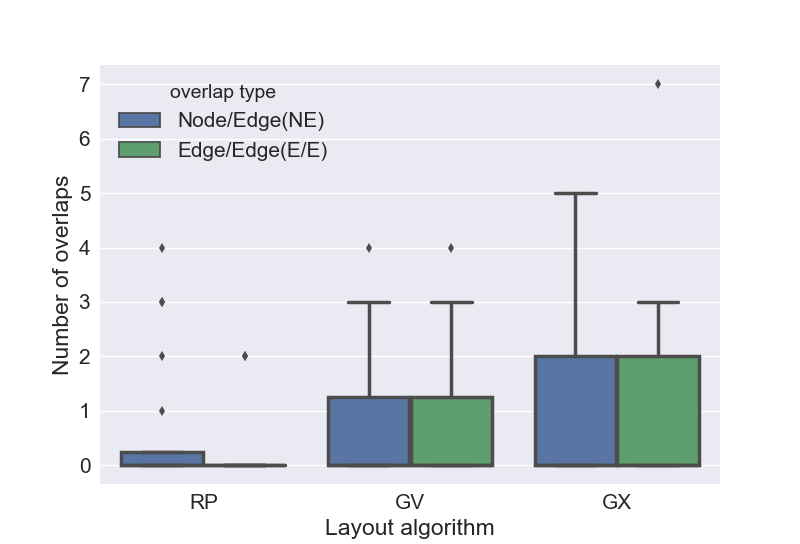
\includegraphics[width=0.9\linewidth]{Evaluation/overlap.png}
	\caption{Overlapping of model elements}
	\label{fig : overlap}
\end{figure}

\begin{figure}
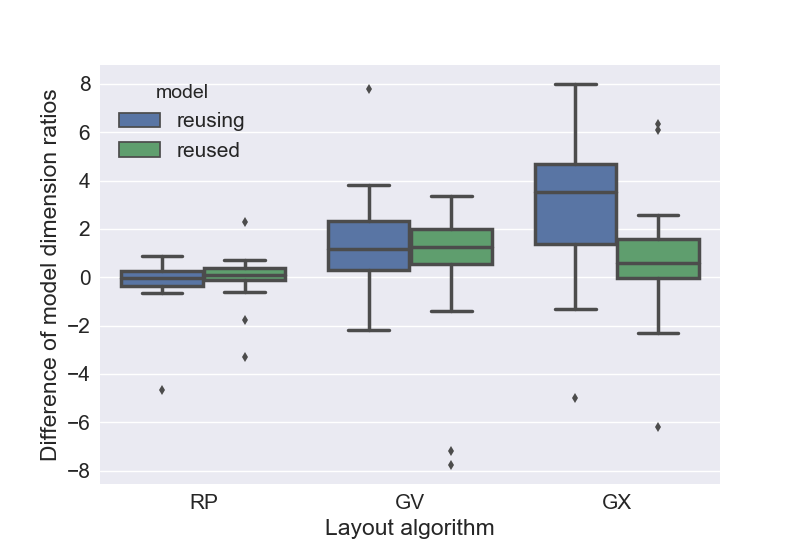
\includegraphics[width=0.9\linewidth]{Evaluation/relativedimension.png}
	\caption{Difference of model dimension ratios}
	\label{fig : relative dimension}
\end{figure}

\begin{figure}
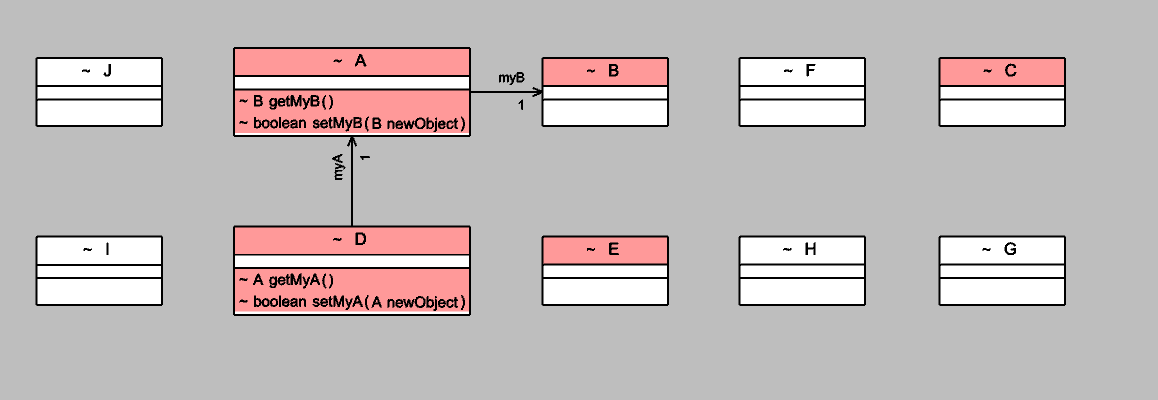
\includegraphics[width=\linewidth]{Evaluation/linksample.png}
	\caption{Element concentrations in merged model}
	\label{fig : links sample}
\end{figure}

\begin{figure}
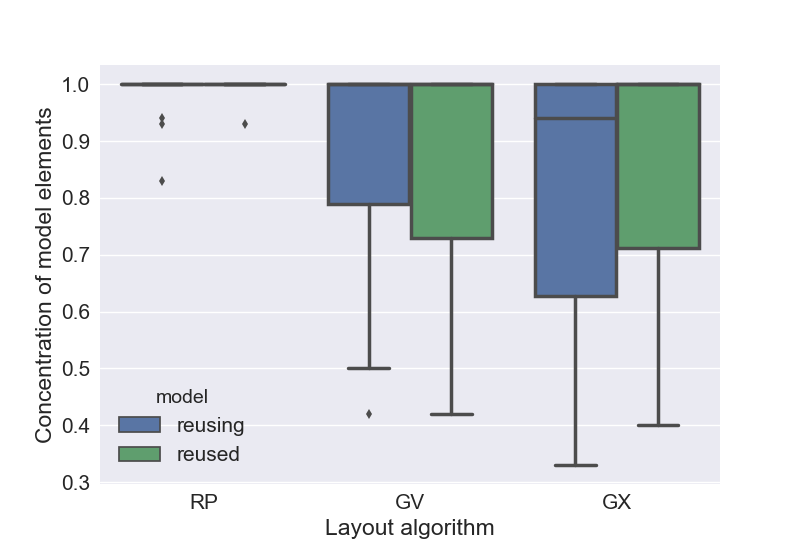
\includegraphics[width=0.9\linewidth]{Evaluation/linkedcomponent.png}
	\caption{Concentration of model elements}
	\label{fig : linked components}
\end{figure}

\begin{figure}
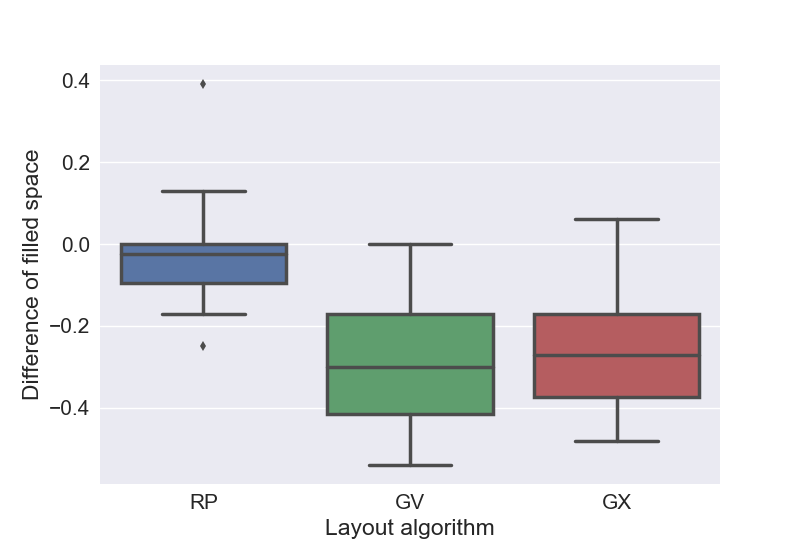
\includegraphics[width=0.9\linewidth]{Evaluation/filledspace.png}
	\caption{Difference of empty space of models}
	\label{fig :Empty Space}
\end{figure}

\begin{figure}
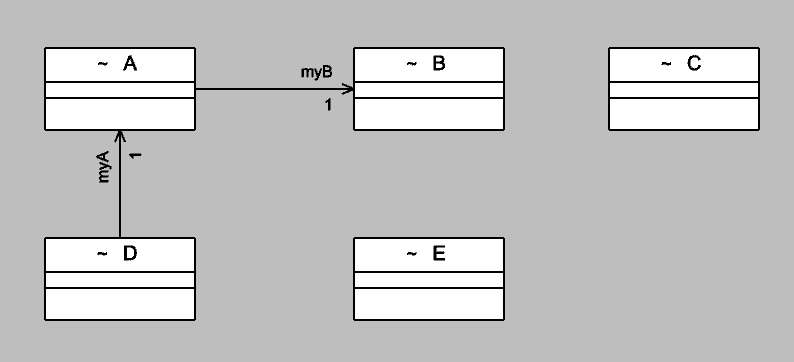
\includegraphics[width=\linewidth]{Evaluation/evaluationfig.PNG}
	\caption{Empty space in model}
	\label{fig : evaluation}
\end{figure}

\textbf{Element concentration.} Furthermore, we evaluate the concentration of the individual model elements from one original model in one place in the merged model. The objective of this is to determine how model elements of one original model are still positioned close to one another after merging. In this regard, we aim to calculate the \haAction{highest} number of adjacent nodes, \haAction{i.e., vertically or horizontally adjacent nodes} in each merged model. Equation \ref{linked equation} shows the formula we employ for this metric.

\begin{equation} \label{linked equation}
  EC = \frac{\haAction{Highest}\ No.\ of\ Adjacent\ Nodes}{Total\ No.\ of\ Nodes}
\end{equation}

For illustration (see Figure \ref{fig : links sample}), the pink colored elements (A, B, C, D, and E) are from the reused model (m2) while the white nodes (E, F, G, H, I, and J) are from the reusing model (m1). Note that node E is a mapped node, therefore, it belongs to both m1 and m2. The optimal value of this metric is 1. Thus, by applying Equation \ref{linked equation}, the \haReplace{adjacent nodes of m1 in the merged model are E, F, H, and G but not I and J, (i.e., the result  is $\frac{4}{6} = 0.67$) while the adjacent nodes of m2  in the merged model are A, B, D, and E but not C (i.e., the result is $\frac{4}{5} = 0.8$).}{ highest number of adjacent nodes of m1 is 4, i.e., (E, F, H, and G) but not 2 (I, and J). Therefore, the result  is $\frac{4}{6} = 0.67$) while the highest number of adjacent nodes of m2 in the merged model is 4, i.e., (A, B, D, and E) but not 1 (C). Hence, the result is $\frac{4}{5} = 0.8$).}  

Figure \ref{fig : linked components} shows the result of this evaluation using the 20 model reuses. The figure shows how the concentration of elements in RP is typically around 1 unlike GV and GX where the concentration is spread over a much wider range. Although, there are outliers in RP with a lowest value at 0.83, this value is still higher than the first quartile of GV and GX. The lowest value in RP is 0.83 while it is just above 0.4 in GV and just above 0.3 in GX, showing that rpGraph keeps the model elements of a model largely close to each other even after they have been combined with other models.

\textbf{Proportion of filled space.} The objective of the filled space metric of a model is to determine how much white space is introduced in the merged model (e.g., an original model placed at the top left while the other original model is at the bottom right with the top right and bottom left quadrants fairly empty). Equation \ref{emptyspace} shows the formula we use to calculate the filled space.

\begin{equation} \label{emptyspace}
  ES = \frac{No.\ of\ Nodes}{Absolute\ No.\ of\ Nodes}
\end{equation}

This metric is illustrated in Figure \ref{fig : evaluation}, where the number of nodes is 5 while the absolute number of nodes is 6 (the empty space below C and to the right of E is counted as another node), resulting in an empty space metric of $\frac{5}{6} = 0.83$. The absolute number is hence the number of nodes that would make the model look like a square or rectangle with all parts filled in with nodes. A node may be counted as two (three, four, ...) if its width or height spans across two (three, four, ...) other nodes. This implies that the maximum value of the metric is 1 with higher values signifying more compact layout. 

In this evaluation, we compare the filled space of a merged model with the filled space of the original models. The average of the original models is used, i.e., the sum of the filled space of reusing and reused models divided by 2. Therefore, 0 means that there is no difference in filled spaces, a positive/negative value indicates that empty space has been reduced/increased in the merged model, respectively. The result of this evaluation is shown in Figure \ref{fig :Empty Space}. The smaller box size of RP whose third quartile is still at 0 indicates the small degree of difference between the compactness of the RP layout and the original layouts compared to GV and GX, whose boxes are wider with their third quartiles close to -0.2. The largest value of RP is 0.15 with an outlier of 0.4, while the maximum value of GV and GX is approximately at 0. The lowest outlier of RP is still higher than the median of GV and GX, with the lowest values of GV and GX going well below -0.4. This evaluation further indicates the robustness of rpGraph in retaining the original layout of models after they have been merged.

\textbf{Similarity of relative positioning.} The last metric verifies the basic premise of the rpGraph algorithm, i.e., the relative positioning of a pair of model elements should not change from the original models to the merged models. Equation \ref{relativepositioning} shows the formula we use to calculate the similarity of relative positioning.

\begin{equation} \label{relativepositioning}
  SRP = \frac{No.\ of\ Pairs\ with\ Similar\ Relative\ Positioning}{Total\ No.\ of\ Pairs\ of\ Nodes}
\end{equation}

Therefore, each pair of nodes in the merged model is compared against the corresponding nodes of the original models. If at least one of the above/below or right/left designations changes from the original model to the merged model, then this pair is not counted for the dividend in Equation \ref{relativepositioning}. As can be seen from Figure \ref{fig :relative positioning}, RP largely retains the relative positioning whereas GV and GX significantly change the relative positioning. Note that the outliers for RP can be explained by anomalies due to a higher number of mappings between model elements of the reusing and reused model. Nevertheless, rpGraph clearly outperforms GraphViz and JGraphX in terms of retaining the original layout.

\begin{figure}
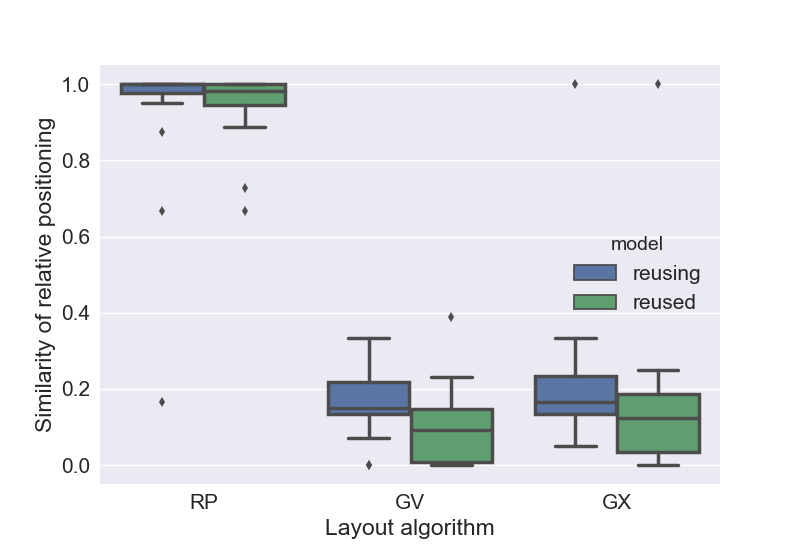
\includegraphics[width=0.9\linewidth]{Evaluation/similarity.png}
	\caption{Similarity of relative positioning}
	\label{fig :relative positioning}
\end{figure}

In summary, additionally to indicating that our rpGraph algorithm largely retains the relative positions of the original model elements, these evaluations also demonstrate that it outperforms GraphViz and JGraphX with regards to overlapping model elements, the retention of model dimension ratios, the continued concentration of individual model elements from the original model, and the occurrence of filled space in the merged models.

\section{Concern Oriented Reuse Layout Using rpGraph} \label{core}
Concern-Oriented Reuse (CORE) is a software reuse paradigm that promotes the use of concern as its main artifact during software development. A concern groups related models (e.g., class diagrams, sequence diagrams, state machines) that cut across software application, and provides three interfaces to facilitate reuse (see Section \ref{concern reuse}). During software reuse, different concern models are \textit{woven/composed} to produce a specific application required for a given a context or domain. In this section, we detail how we use rpGraph to layout the combined model diagrams of a concern. First, we give a structural overview of a concern and then present the layout algorithm of a concern models using rpGraph.

\subsection{Concern Structure}
The basic structure of a concern is shown in the excerpt of the metamodel in Figure \ref{fig : core metamodel}. A concern (\textit{COREConcern}) groups related models (\textit{COREModel}) together, with at least one model by default. A COREModel is an abstract class which is concretely defined via sub-classing (\textit{corification}). Several models including class diagram, sequence diagram, state machine, and aspects can be corified, i.e., making them to behave like concern models (\textit{COREModel}). In this work, we use corified Reusable Aspect Model (RAM) to demonstrate the application of rpGraph in a layout of merged concern models.  A concern is composed of one feature model (\textit{COREFeatureModel}), see Figure \ref{fig : core metamodel}, a subclass of COREModel. A feature model groups the commonality and variations of a family of software products such as authentication, logging, and authorization. Each software artifact in a family is represented as a feature (\textit{COREFeature}). A feature is realized by one or more COREModels, conversely, a COREModel can realize one or more core features. The classes with pink background in Figure \ref{fig : core metamodel} depicts the structure through which concern models are reused, which is not the main focus of this work.

\begin{figure}
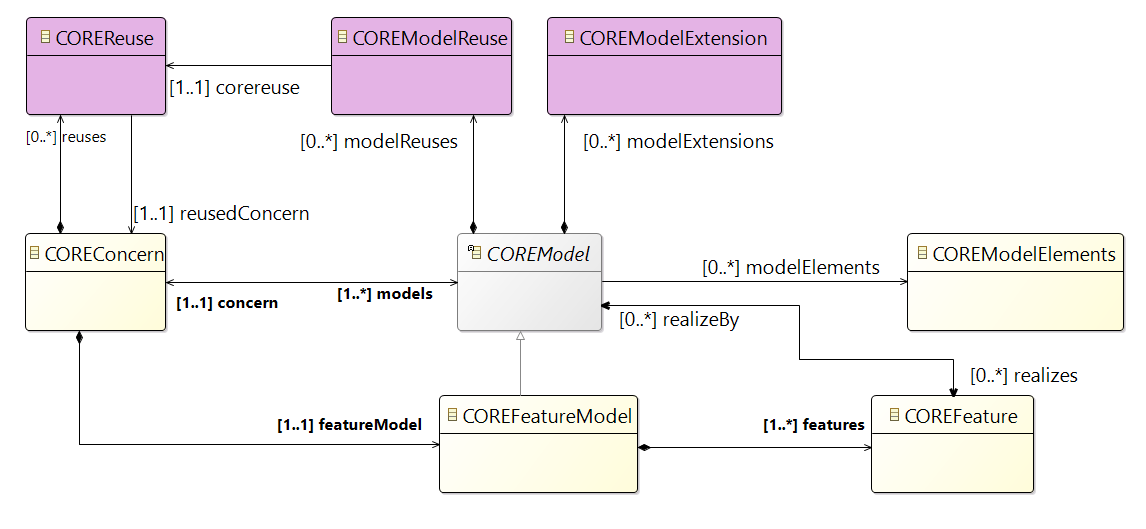
\includegraphics[width=\linewidth]{coremetamodel.PNG}
	\caption{Basic Structure of a Concern}
	\label{fig : core metamodel}
\end{figure}

\subsection{CORE Feature Model and Weaving Algorithm} \label{fm and weaving}
Feature Model is a tree diagram that specifies the commonalities and variabilities of a set of features belonging to a particular domain. The main objective of feature model is to enhance reuse during software development. A simple example of a feature model is an authentication as shown in Figure \ref{fig : authentication fm}. The feature model has a root feature, Authentication, and several sub-features as shown in the Figure. This feature model groups different authentication means with Password being compulsory, denoted by black filled bulb. Based on a feature selection (\textit{Configuration}), different authentication means can be configured from the feature model, e.g., Password and Biometric, Password and Access Card, or Password, Biometric and Access Card. A feature model represents the variation interface of a concern. Each feature (e.g., Password) has a realization model as shown in the metamodel, Figure \ref{fig : core metamodel}. Based on a particular configuration, the realization models of the selected features are combined together to produce a more compact and concise model of the concern, (\textit{Weaving}). 

In CORE, bottom-up weaving algorithm is used, i.e., the composition of the selected models start from the the highest level of the feature model. Feature model is arranged in levels with root feature being level 1. As shown in Figure \ref{fig : authentication fm}, the highest level is 3. If all features are selected during the concern reuse, the realization models of Facial Recognition (FR), Retina Scan (RS), Bar Code (BC), Magnetic, Biometric, Password, Access Card (AC), and Authentication are combined to produce one model.  Facial Recognition, Retina Scan, Bar Code, and Magnetic being at level 3 are combined first in any order, two models during each iteration.  The next models to merge are are Biometric, Password, and Access Card (level 2), and finally Authentication which is at level 1.  Each composition (merging of two models) produces a merged model which is combined with subsequent models.  In each case, a merged model is produced and the trends continues until all the realization models of the selected features are woven together. The composed model of the seven(8) software artifacts produces the required authentication concern based on the configuration. It is essential that the layout of the woven model retains the original layout information of the individual models which is currently lost with existing automatic layout mechanisms, e.g., GraphViz, and JGRaphX. In the next section, we show how we apply rpGraph to address this challenge.
  \begin{figure}
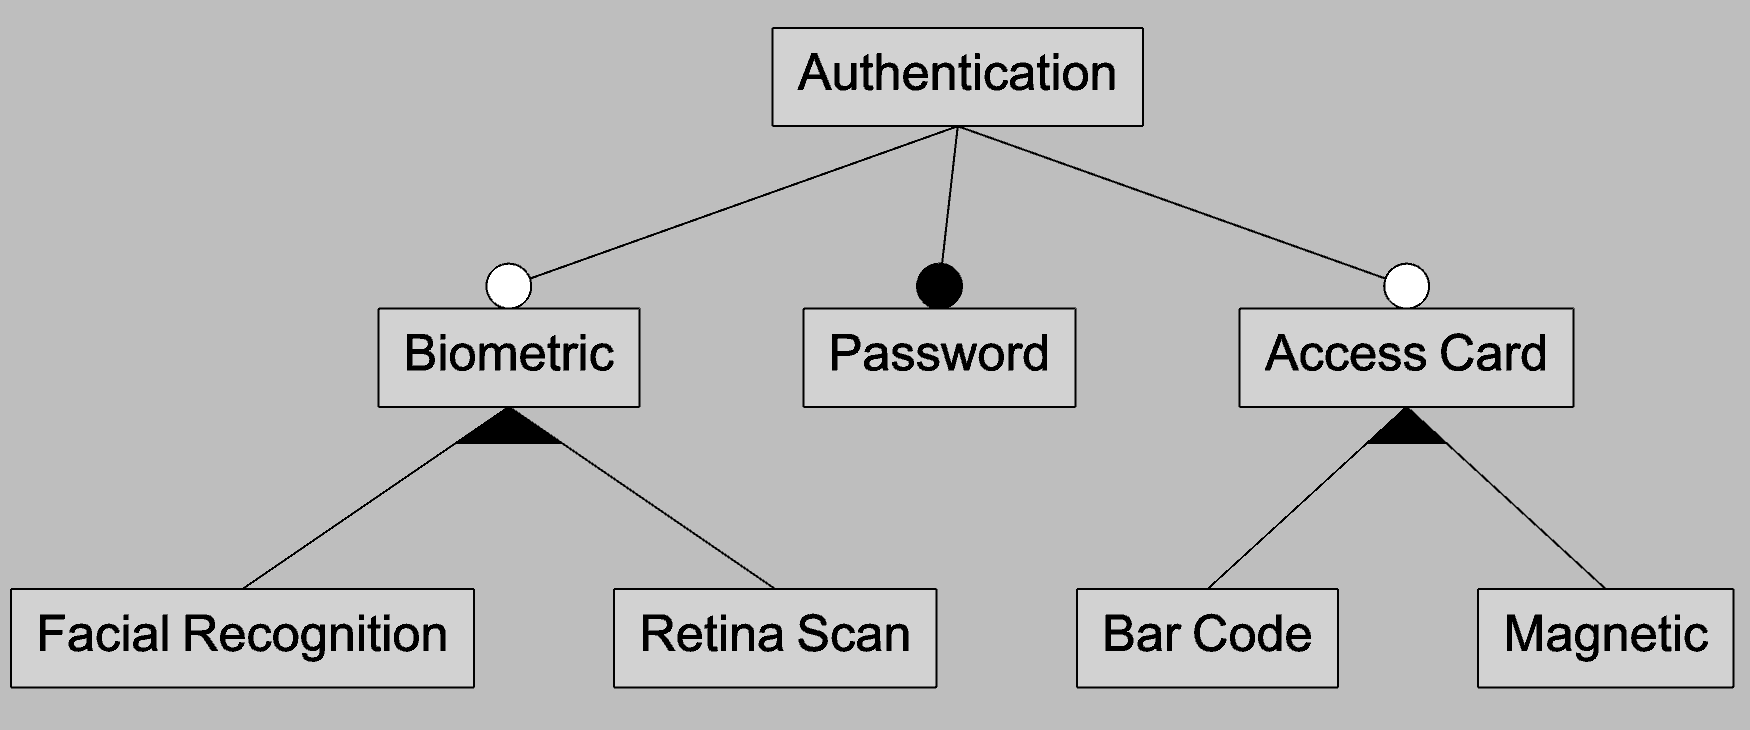
\includegraphics[width=\linewidth]{authenticationfm.PNG}
	\caption{Basic authentication feature model.}
	\label{fig : authentication fm}
\end{figure}

\subsection{Concern Layout Algorithm Using rpGraph}
This section describes the layout of a concern, i.e., a woven model, using rpGraph. This algorithm is strictly based on the weaving techniques of CORE, (see Section \ref{fm and weaving}, in addition to the formalisms provided by the rpGraph (see Section \ref{rpGraph algorithm}, and is implemented in the TouchCORE tool (see Section \ref{touchcore}). The following subsections detail the algorithm.
\begin{figure}
	\centering
    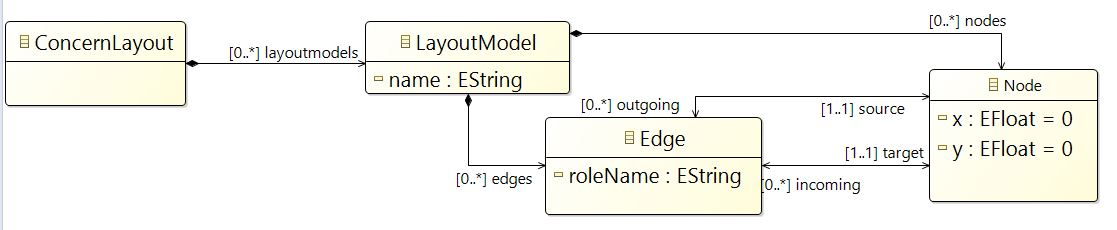
\includegraphics[width=1\linewidth]{concernlayout.JPG}
    \caption{Concern layout metamodel (Excerpt shown)}
    \label{fig : concern layout metamodel}
\end{figure}
\subsubsection{Create Concern Layout}
The rpGraph layout metamodel has been modified to support the Concern-Oriented Layout, excerpt shown in Figure \ref{fig : concern layout metamodel}. During each composition, each of the two RAM models maintained by the TouchCORE tool is used to create a LayoutModel, (see Section \ref{create layout model}), except that the edges are not assigned at this juncture. The ConcernLayout which is composed of LayoutModel is updated after each composition. Before the first composition, TouchCORE creates an empty concern where all the selected artifacts are woven into. In this work, we regard the empty concern as the reusing model while each realization model during  each composition is seen as a reused model. Hence, the updates of the concern layout models involves layout  modification of existing model elements (i.e., reusing model elements, if any), and addition of new model elements (reused model elements). For example, if the first composition using the authentication feature model (see Figure \ref{fig : authentication fm}) is Facial Recognition,  it is then woven into the empty authentication concern. This composition involves only one model and hence no merging, but the layout model of the reused model (in this case, Facial Recognition) is added to the empty concern layout during the composition. Next composition could be Magnetic against the authentication concern, which currently contains only Facial Recognition. Hence, the concern model is updated to reflect the original layout information (i.e., the layout status produced by rpGraph during the previous composition)  before the second composition. This update is essential because TouchCORE tool arbitrarily rearranges the layout information during each composition.  The Magnetic model is only added to the authentication concern during the layout composition because the Magnetic model has no relationship with the Facial Recognition, i.e., no mapping between the two models. Therefore, no merging is required. In TouchCORE, mapping between model elements can be manually specified  or inherently mapped between two classes with the same name.  The next section details the layout algorithm of a concern using rpGraph.

\subsubsection{Reposition the Concern Layout with rpGraph}
 In this section, we detail how we reposition the layout information of the concern models. The overall algorithm is shown in Figure \ref{concern layout overview}
  \begin{figure}
	\centering
    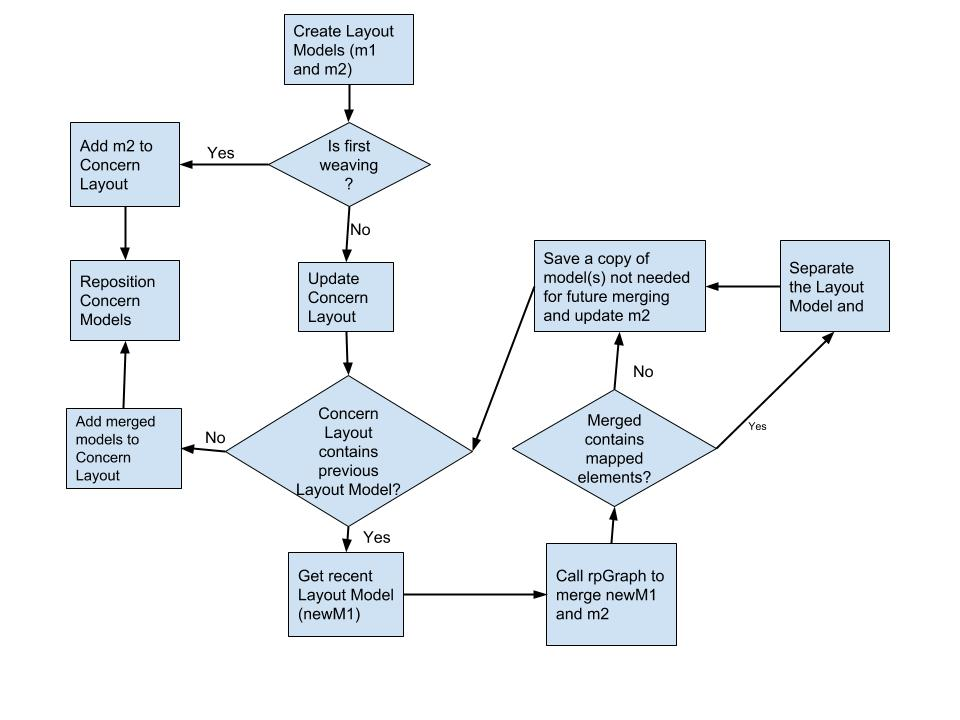
\includegraphics[width=1\linewidth]{concernOverview.jpg}
    \caption{Concern layout overview}
    \label{concern layout overview}
\end{figure}

 \begin{figure}
	\centering
    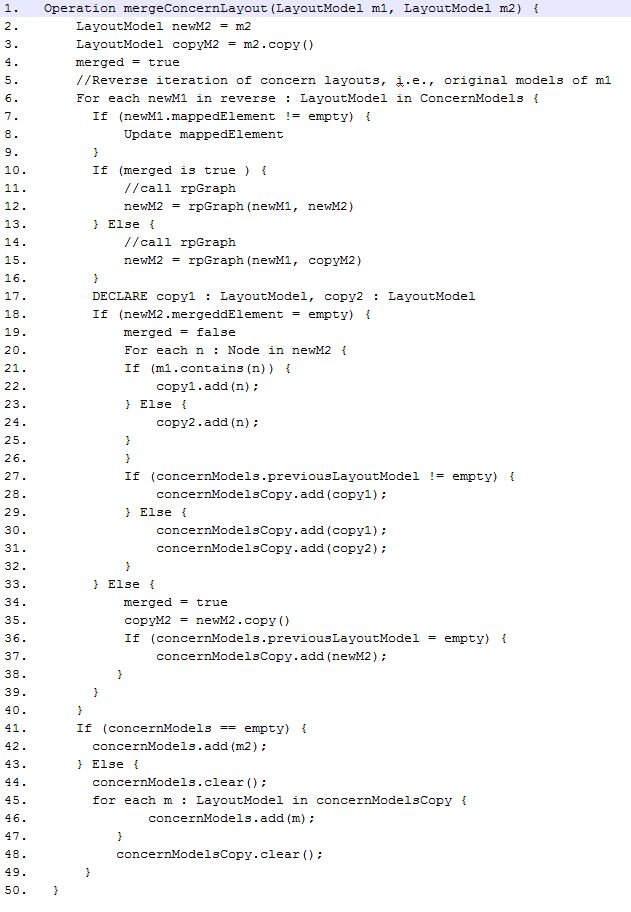
\includegraphics[width=1\linewidth]{concernalgorithm.JPG}
    \caption{Concern layout algorithm}
    \label{fig : concern algorithm}
\end{figure}

\subsubsection{Merge Concern Layout Models}
%It is evident at this juncture that the number of concern models increases proportionally with the number of composition. 
In this section, we describe how we merge concern models to retain its original layout information using rpGraph. The operation "mergeConcernLayout(m1, m2)" handles the repositioning algorithm (see Figure \ref{fig : concern algorithm} for the complete merging algorithm). The two models : m1 and m2, are to be merged during each composition.  According to the weaving algorithm in ToucCORE (see Section \ref{fm and weaving}), the resulting model of a composition, represented by m1, is used as an input model for the next weaving and so on. In the first place, m2, which is the reused model, is assigned to a LayoutModel variable, newM2, and a copy of m2 is also created, copyM2, (lines 2-3 in Figure \ref{fig : concern algorithm}). The newM2 is used in place of m2, and it undergoes several changes as each original model of m1, i.e., the realization models that have been woven before, is combined with it. The copy of m2 is needed during models merge that requires original layout information of m2. The variable, "concernModels" is a list of LayoutModel (see Figure \ref{fig : concern layout metamodel}) that have been combined together . During each composition, the concernModels is traversed in reverse direction, i.e., LIFO - Last In First Out, one model is retrieved at a time, newM1, and is merged with either newM2 or copyM2 using the rpGraph (lines 6-16 in Figure  \ref{fig : concern algorithm}). The result of this merge always returns a model, newM2 (lines 12 and 15 in Figure \ref{fig : concern algorithm}). If the two combined models do not have direct relationship such as mapped elements or parent/child relationship, they are not merged, instead, the models are kept apart in newM2 model, i.e., newM2 contains the two separate models. In this case, newM2 is separated into copy1 (m1 elements), and copy2 (m2 elements), (lines 17-26 in Figure  \ref{fig : concern algorithm}). Further, we check if "concernModels" has another model to be combined with newM2(line 27 in Figure  \ref{fig : concern algorithm}). If next composition exist, "copy1" is stored in a list variable "concernModelsCopy", (lines 27-29 in Figure  \ref{fig : concern algorithm}), which holds models that are not needed for subsequent composition(s). Otherwise,  both copy1 and copy 2 are stored in concernModelsCopy, (lines 29-32 in Figure  \ref{fig : concern algorithm}).  This concernModelsCopy is used to update the concernModels after all the compositions. On the other hand, newM2 might have mapped elements or contains parent/child models. Therefore, the model contents of newM2 is not separate. Hence, newM2 is added to concernModelsCopy if it is the last composition (lines 33-40 in Figure  \ref{fig : concern algorithm}). Whenever a composition produces a merged model that contains mapped elements, copyM2 is updated to have the same layout information as the resulting model.  This ensures that when an original layout information of m2 is required, i.e., when newM2 contains separate models during composition, copyM2 model is used instead. The idea is that once there is a merged model with mapped elements, the result becomes the original model of m2. During each subsequent composition, newM2 is used if the previous composition produced model with mapped elements, else, copyM2 is used. In either case, newM1 is used (lines 10-16 in Figure  \ref{fig : concern algorithm}). This iteration continues until all the concern models have been woven into newM2.

The next step is to update the concernModels before the concern layout is repositioned. During the first composition, the m2 is weaved into empty concern. Hence, the concern model is empty and no model is merged. Instead, m2 is added to concern models, (lines 41-43 in Figure  \ref{fig : concern algorithm}). However, for subsequent composition, the concernModels is updated to reflect the current status of the concern layout (lines 43-49 in Figure  \ref{fig : concern algorithm}). Finally, the layout information of the concern model elements are updated to reflect the changes.

\subsection{Concern Layout Examples}
In this section, we illustrate the layout of concern models using rpGraph, and visually compare our results with related layout solutions,  GraphViz and JGraphX. Figure \ref{basicConfig} depicts feature selection (\textit{feature configuration}) of a basic feature model with one root feature and two leaf/children features. Following the configuration is the combination of the realization models of the features, each realization model is shown in Figure \ref{basic realizing models}. The layout of the combined model using rpGraph is shown in Figure \ref{rpBasic} while Figure \ref{gvBasic} and \ref{gxBasic} depict the same combined model using GraphViz, and JGraphX, respectively.  In each woven model, there is tracing display with different colour background, each represents a given feature whose model was woven into the concern. Using the tracing information, it is very clear that rpGraph retains the original positions of each individual model elements after the compositions. GraphViz, and JGraphX rearrange the model elements and the mental map of each individual model is completely lost.
\begin{figure}
	\centering
    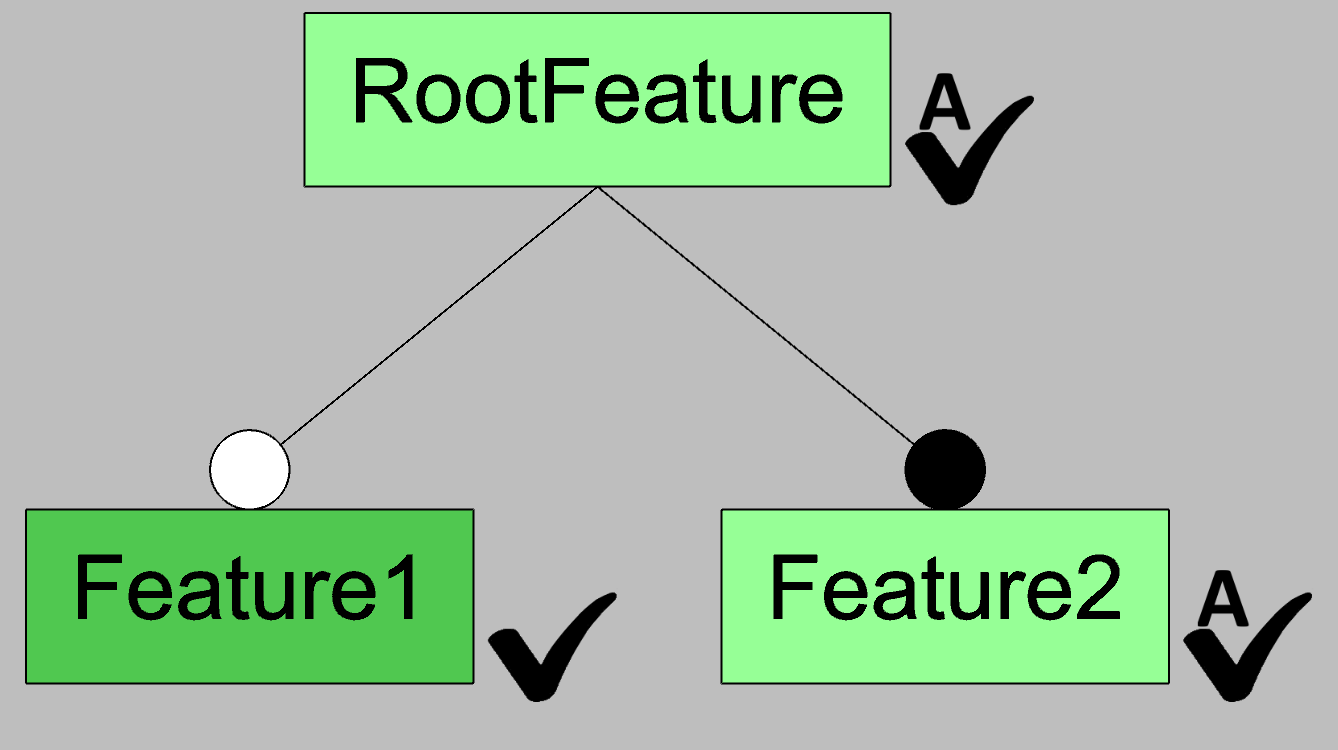
\includegraphics[width=1\linewidth]{exfm.PNG}
	\caption{Basic configuration of feature model}
    \label{basicConfig}
\end{figure}
\begin{figure}
	\centering
    \begin{subfigure}[b]{0.3\linewidth}
    	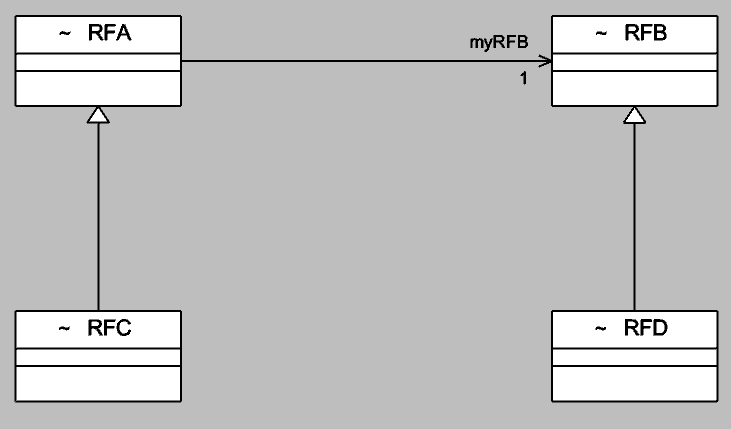
\includegraphics[width=\linewidth]{rootfeature.PNG}
        \caption{Root feature}
        \label{rootfeature}
    \end{subfigure}
    \begin{subfigure}[b]{0.3\linewidth}
    	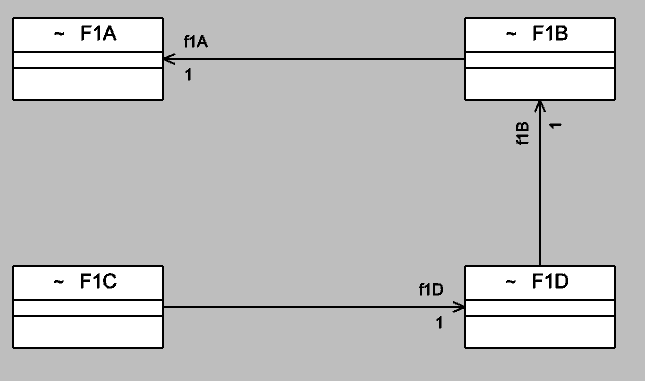
\includegraphics[width=\linewidth]{feature1.PNG}
        \caption{Feature 1}
        \label{feature1}
    \end{subfigure}
    \begin{subfigure}[b]{0.3\linewidth}
    	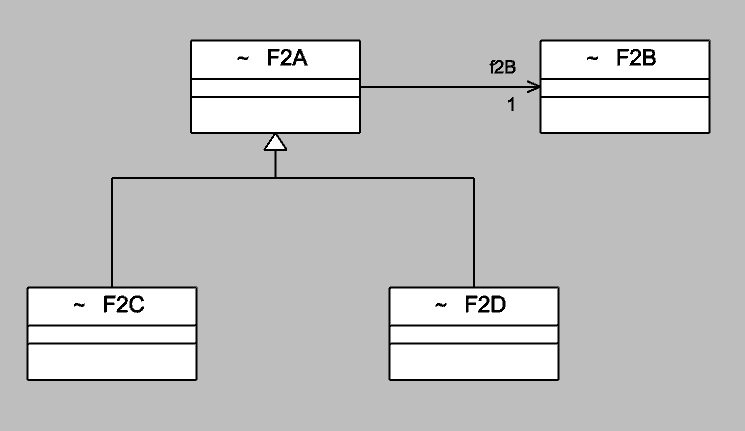
\includegraphics[width=\linewidth]{feature2.PNG}
        \caption{Feature 2}
        \label{feature2}
    \end{subfigure}
	\caption{Realizing models of Figure \ref{basicConfig}}
    \label{basic realizing models}
\end{figure}

\begin{figure}
	\centering
    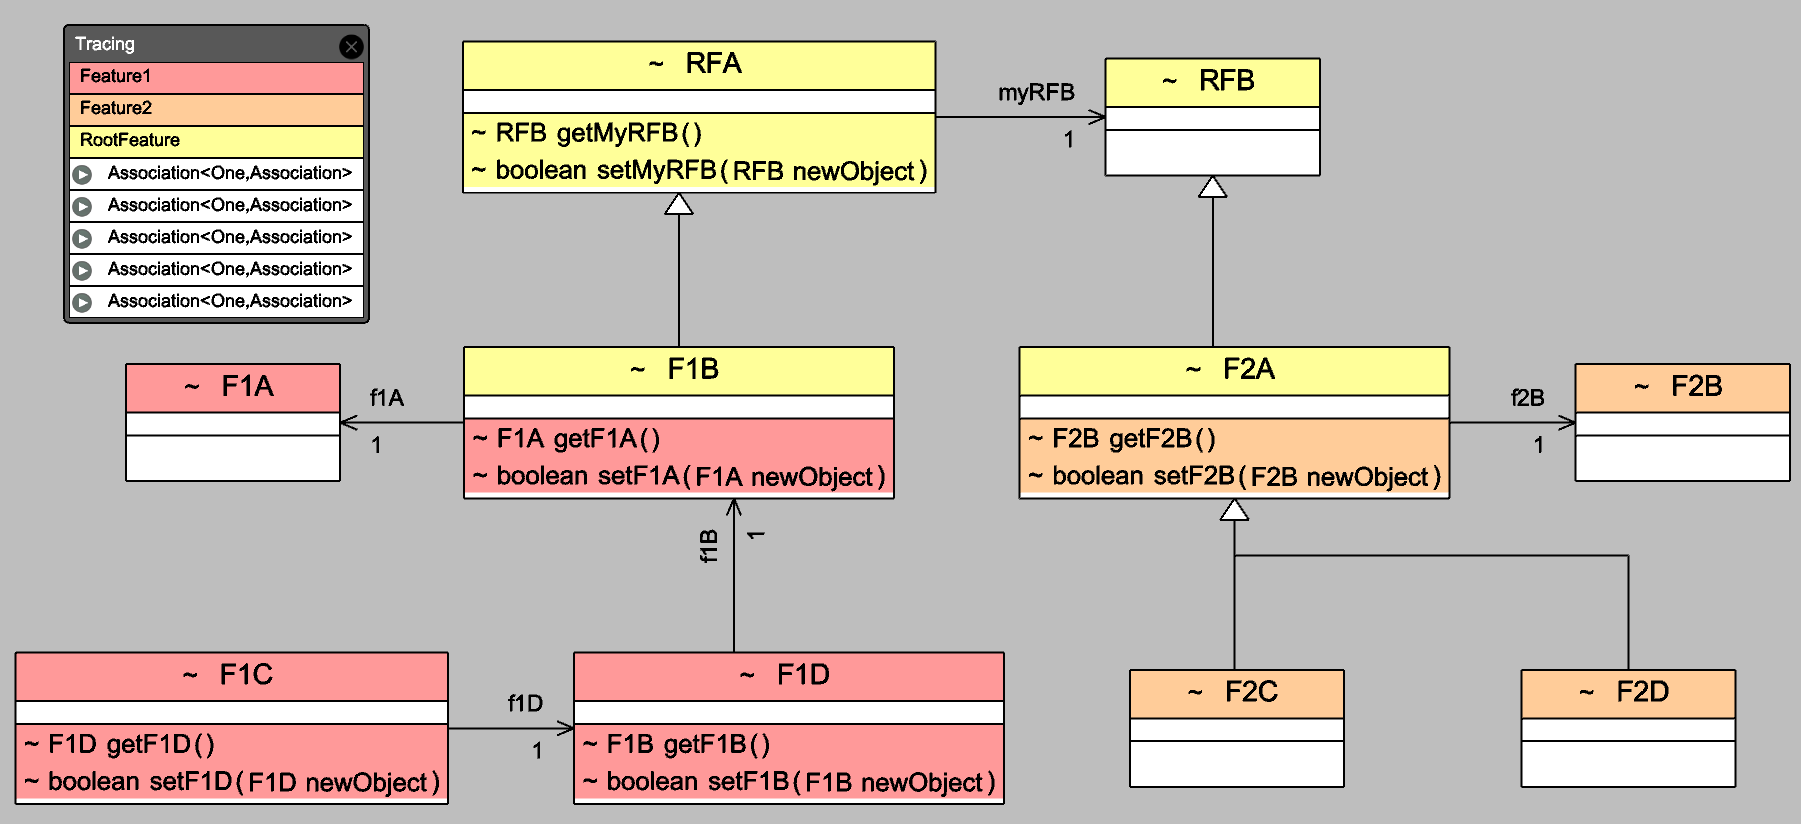
\includegraphics[width=1\linewidth]{exrp.PNG}
	\caption{Layout of the basic feature model using rpGraph}
    \label{rpBasic}
\end{figure}
\begin{figure}
	\centering
    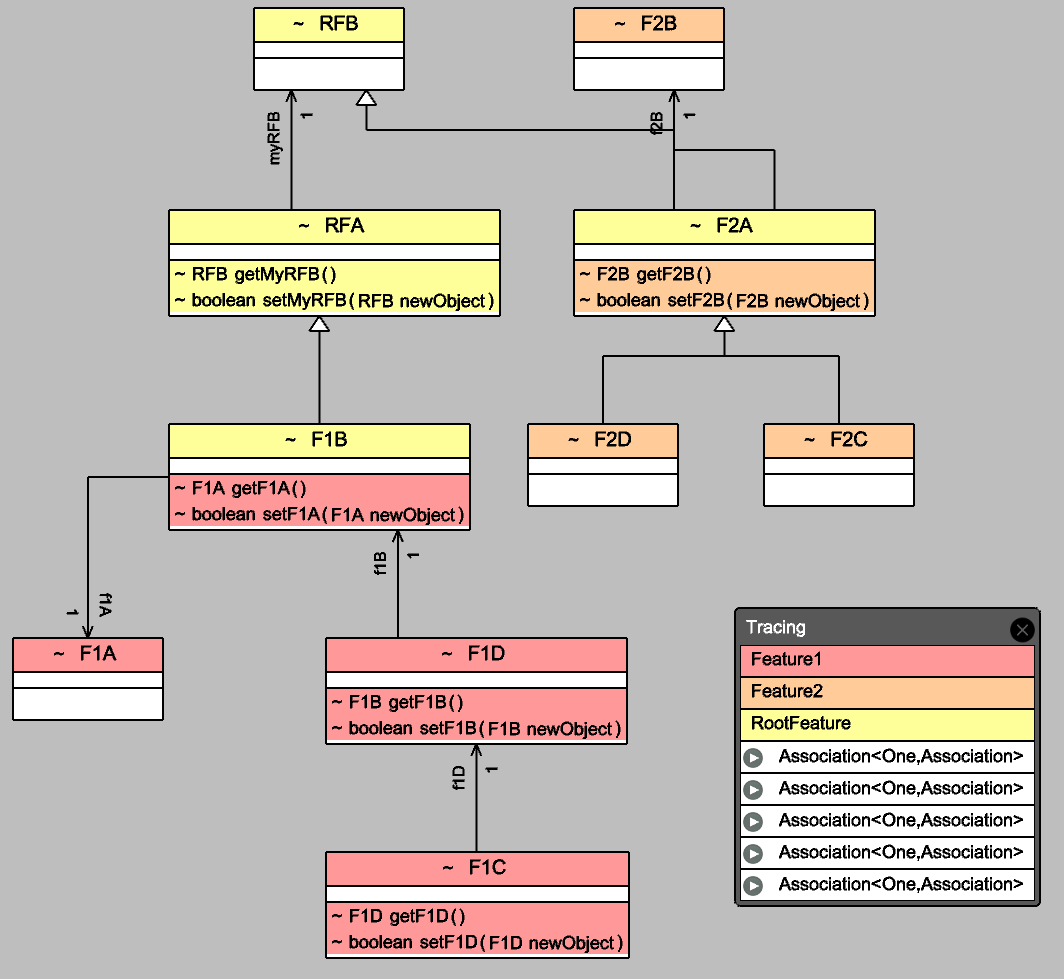
\includegraphics[width=1\linewidth]{exgv.PNG}
	\caption{Layout of the basic feature model using GraphViz}
    \label{gvBasic}
\end{figure}
\begin{figure}
	\centering
    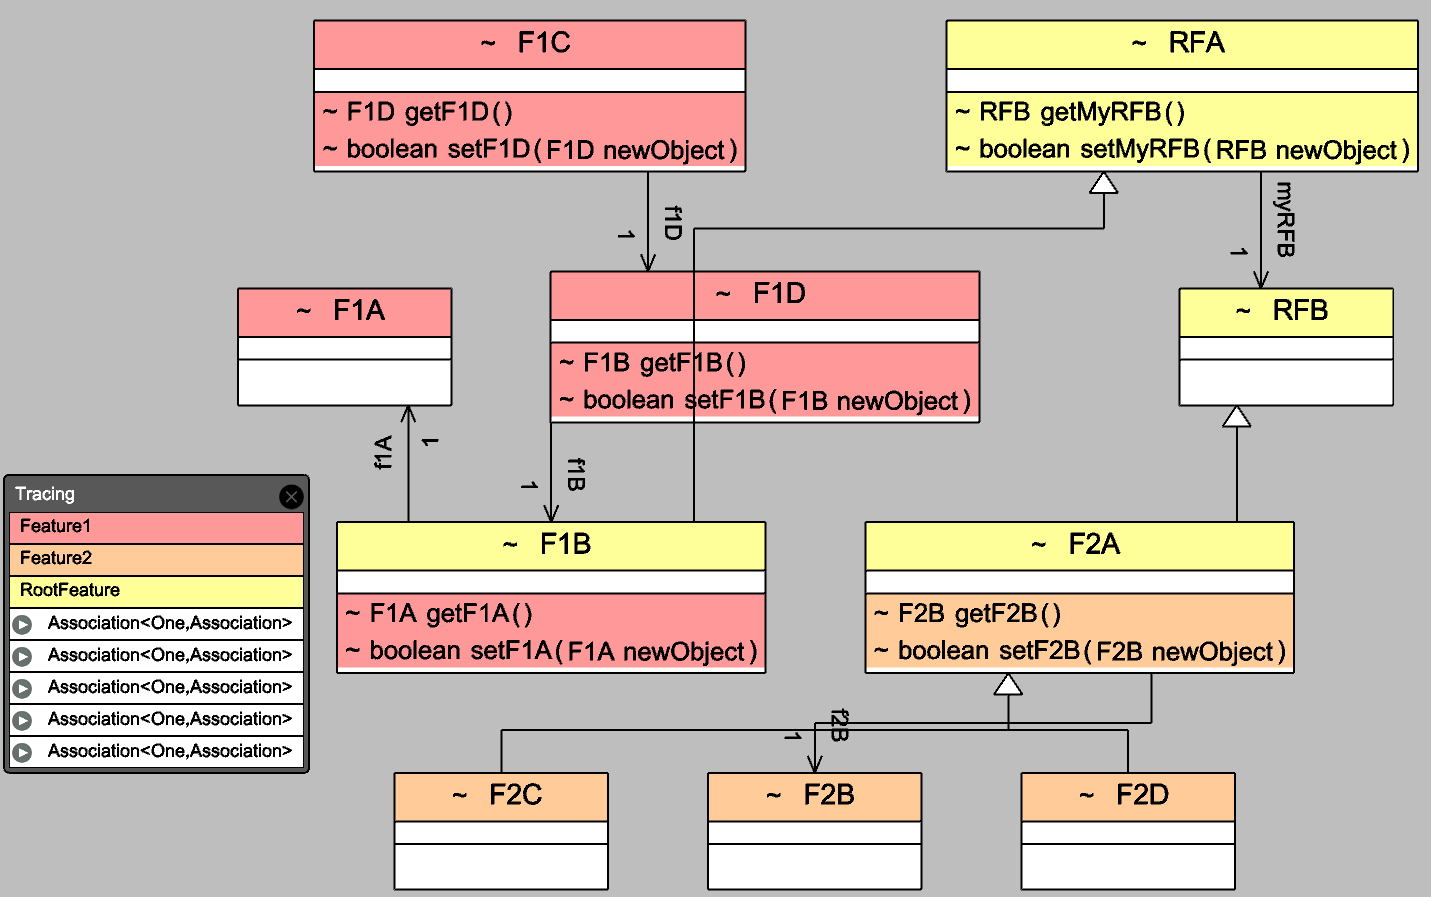
\includegraphics[width=1\linewidth]{exgx.PNG}
	\caption{Layout of the basic feature model using JGraphX}
    \label{gxBasic}
\end{figure}

Another illustration is the layouts of different authentication configurations. The authentication concern has different features used to realize various means of authentication as shown in Figure \ref{authenticationExampl}.  For illustration, a configuration of the authentication concern with the following features: Access Blocking, AuthenticationMeans (Password, Facial Recognition, and Magnetic Card), and Auto Logoff as shown in Figure \ref{authentication configuration}. The realization models of the selected features are shown in Figure \ref{basic realizing models}, except features without realization model such as AuthenticationMeans, Biometric, and Technology. They are used for structural grouping in the feature model.

\begin{figure}
	\centering
    \includegraphics[width=1\linewidth]{authenticationConcern.PNG}
	\caption{Feature model oF authentication with different authentication means.}
    \label{authenticationExampl}
\end{figure}
\begin{figure}
	\centering
    \includegraphics[width=1\linewidth]{biopasswordcardfm.PNG}
	\caption{Configuration of authentication concern}
    \label{authentication configuration}
\end{figure}

\begin{figure}
	\centering
    \begin{subfigure}[b]{0.3\linewidth}
    	\includegraphics[width=\linewidth]{authenticationModel.PNG}
        \caption{Authentication model.}
        \label{authentication model}
    \end{subfigure}
    \begin{subfigure}[b]{0.3\linewidth}
    	\includegraphics[width=\linewidth]{accessblockingModel.PNG}
        \caption{Access blocking model.}
        \label{access blocking}
    \end{subfigure}
    \begin{subfigure}[b]{0.3\linewidth}
    	\includegraphics[width=\linewidth]{autologoffModel.PNG}
        \caption{Auto Logoff model}
        \label{auto logoff}
    \end{subfigure}
    \begin{subfigure}[b]{0.3\linewidth}
    	\includegraphics[width=\linewidth]{facialrognitionModel.PNG}
        \caption{Facial Recognition model.}
        \label{facial recognition}
    \end{subfigure}
    \begin{subfigure}[b]{0.3\linewidth}
    	\includegraphics[width=\linewidth]{passwordModel.PNG}
        \caption{Password model.}
        \label{password model}
    \end{subfigure}
    \begin{subfigure}[b]{0.3\linewidth}
    	\includegraphics[width=\linewidth]{cardModel.PNG}
        \caption{Aceess Card model}
        \label{access card}
    \end{subfigure}
    \begin{subfigure}[b]{0.3\linewidth}
    	\includegraphics[width=\linewidth]{magneticModel.PNG}
        \caption{Magnetic model}
        \label{magnetic}
    \end{subfigure}
	\caption{Realization models of Figure \ref{authentication configuration}}
    \label{basic realizing models}
\end{figure}

When these models are composed according to the weaving algorithm in TouchCORE, and using rpGraph to reposition the layout, the original positions of the individual model elements are maintained (see Figure \ref{authentication with rpGraph}). However, it is obvious that GraphViz, and JGraphX distort the layout information of the original models in the merged model to the extent some salient layout information is lost and the overall of each model disorganized, (see Figure \ref{authentication with GraphViz}, and \ref{authentication with JGRaphX}).

\begin{figure}
	\centering
    \includegraphics[width=1\linewidth]{biopasswordcardrp.PNG}
	\caption{Layout of woven Figure \ref{authentication configuration} using rpGraph}
    \label{authentication with rpGraph}
\end{figure}
\begin{figure}
	\centering
    \includegraphics[width=1\linewidth]{biopasswordcardgv.PNG}
	\caption{Layout of woven Figure \ref{authentication configuration} using GraphViz}
    \label{authentication with GraphViz}
\end{figure}
\begin{figure}
	\centering
    \includegraphics[width=1\linewidth]{biopasswordcardgx.PNG}
	\caption{Layout of woven Figure \ref{authentication configuration} using JGraphX}
    \label{authentication with JGRaphX}
\end{figure}


\section{Results and Discussion, \textit{Concern Oriented Reuse Layout}}\label{concern discussion}
In this section, we further evaluate our rpGraph algorithm by comparing its layout of merged concern models with GraphViz (GV), and JGraphX (GX). In this evaluation, we also denote our algorithm as Relative Positioning (RP). We use two existing concern realization models (class diagrams) from the TouchCORE library of concern models. The concerns are Authentication with 14 sub-features, and Workflow with five sub-features. In total, we evaluate 20 different configurations, i.e, 20 different feature selections based on the Authentication, and Workflow concerns.  The number of classes in each composed models ranges from 9 to 25. The number of pairs of mapped classes used in each two combined models spans from from 1 to 3. All the original and merged models used in this evaluation are available in the rpGraph GitHub repository\footnote{The concern feature model, realization model of each feature, and merged models of each configuration with rpGraph, GraphViz, and JGraphX can be found in GitHub, https://github.com/Hyacinth-Ali/AutoLayoutDataset/tree/master/LayoutImages. The \textit{Tracing} information uses different colour to distinguish among different model elements. The name of the models \_RP, \_GV, and \_GX correspond to the layout of rpGraph, GraphViz, and JGraphX, respectively}. 

 In the remainder of this section, we discuss the results of the different layout algorithms of concern models using the same metrics as illustrated in Section \ref{discussion}. Similarly, the evaluation is rooted in the assumption that the modeler's mental map of the original models is least disrupted, if the layout does not change. This involves, among others, the retention of the original positions of the concern model elements after combining the models. 

\textbf{Overlapping model elements.} In overlapping of model elements, least value signifies better performance. Figure \ref{concern overlap} shows the box plot of the number of overlaps which summarizes its distribution.  While the median number of NE overlaps in RP mechanism is 0, GX and GV are approximately at 1. Although, the third quartile of NE in GV is below RP at 2, both GX and GV have EE third quartile approximately at 2 while RP is at 0.  In overall, third quartile of GV has a smaller number of overlaps for NE (1.2), while third quartile of RP has smallest number of EE at 0 but with one outlier at 1. The outlier is still far below the third quartile of EE in GX and GV indicating better performance of rpGraph for EE..

\textbf{Difference of model dimension ratios.}  In this evaluation, we aim to determine how the model dimension ratio of each original model is retained after the composition of the concern models. Hence, the difference between the "before" and "after"  ratio of each algorithm is calculated. Figure \ref{concern model ratio} shows the distribution of the difference in the concern model dimension ratios. The small gap between first and third quartiles of RP compared to GV and GX indicates that RP better maintains the model dimension ratio of each model. In detail, the gap between first and third quartiles of RP in root feature is predominantly very small, about 0.4 to 0.8, compared to the root feature of the other two mechanisms whose gaps span from -0.43 to -0.17. This excellent performance of rpGraph is attributed to the higher priority given to the root feature during composition. Considering other models, the gap between first and third quartiles of RP is still smaller (-0.17 to 0.02), compared to the other two which ranges from -0.45 to 0.03. In overall, the median value of RP for both root feature and other models are very close to 0 compared to GX and GV.  The extreme values for RP are -0.6 (root feature) and -8(other models) compared to -5 and -14 in GX, and -7.5 and -11.5 in GV, respectively. In overall, rpGraph outperforms the other layout mechanisms in retaining the dimensions of the layouts of the original concern models.

\begin{figure}
\includegraphics[width=0.9\linewidth]{Evaluation/overlap_Concern.png}
	\caption{Overlapping of concern model elements}
	\label{concern overlap}
\end{figure}

\begin{figure}
\includegraphics[width=0.9\linewidth]{Evaluation/modelratio_Concern.png}
	\caption{Difference of concern model dimension ratios}
	\label{concern model ratio}
\end{figure}

\begin{figure}
\includegraphics[width=0.9\linewidth]{Evaluation/linked_Concern.png}
	\caption{Concentration of model elements}
	\label{concern linked components}
\end{figure}


\begin{figure}
\includegraphics[width=\linewidth]{Evaluation/filledspace.png}
	\caption{Proportion of filled space in concern model}
	\label{concern filled space}
\end{figure}

\textbf{Element concentration.}  Furthermore, we evaluate the concentration of the individual model elements from one original model in one place in the composed concern model. The objective of this is to determine how model elements of one original model are still positioned close to one another after the composition of concern models. The algorithm is the same as one used in Section \ref{discussion}, using the same equation \ref{linked equation}

Figure \ref{concern linked components} shows the result of this evaluation using the 20 different feature configurations. The figure shows how the concentration of root feature elements in RP is typically around 1 unlike GV and GX where the root feature concentration is spread over a much wider range of 1 to 0.9, and 0.8 to 0.65, respectively. Considering other models, the media of RP is typically at 0 compared to GX and GV at 0.7 and 0.8, respectively. Similarly, the first quartile of RP is less than the other two. In overall, the values of each first and median values in RP is more than the corresponding values in GX and GV  showing that rpGraph keeps the model elements of a model largely close to each other even after they have been combined with other models.

\textbf{Proportion of filled spaces.} In this evaluation, we compare the filled space of a merged model with the filled space of the original models. The average of the original models is used, i.e., the sum of the filled space of the selected realization models divided by number of features selected. The result of this evaluation is shown in Figure \ref{concern filled space}. The third quartile of RP at 0.3, is significantly less than the median values of GX and GV at 0.36 and 0.34, respectively. Moreover, the first quartile of RP (0.1) is far less than the corresponding first quartile of GX (0.3) and GV(0.18). The largest value of RP is 0.3, while the maximum value of GV and GX is approximately at 0.42. This evaluation further indicates the robustness of rpGraph in retaining the original layout of models after they have been composed together.

\textbf{Similarity of relative positioning.} In this evaluation, each pair of nodes in the merged model is compared against the corresponding nodes of the original models.  As can be seen from Figure \ref{concern relative positioning}, The overall shape of root feature in RP is predominantly around 1 compared to GX and GV with third quartile at 0.2 and 0.5, respectively. RP largely retains the relative positioning whereas GV and GX significantly change the relative positioning. Note that the few outliers for root feature RP can be explained by anomalies due to a higher number of mappings among the realization models. Although, we give higher priority to the root feature model, the relative positioning of other models in RP still outperform GX and GV.  The first quartile value of RP is 0.5 while the third quartile values of GX and GV are at 0.5 and 0.26, respectively.

\begin{figure}
\includegraphics[width=0.9\linewidth]{Evaluation/similarity_Concern.png}
	\caption{Similarity of concern relative positioning}
	\label{concern relative positioning}
\end{figure}

In summary, additionally to indicating that our rpGraph algorithm largely retains the relative positions of the original model elements in a composed concern model, these evaluations also demonstrate that it outperforms GraphViz and JGraphX with regards to overlapping (Edge/Edge) model elements, the retention of model dimension ratios, the continued concentration of individual model elements from the original model, and the occurrence of filled space in the merged models.

\section{Threats to validity}\label{threats to validity}
The data used in this evaluation is from software engineering lab at McGill University. The result of the evaluation may vary when when more data from varieties of domain are used for the evaluation. Another issue that might impact the outcome of the result is the process of the evaluation. One person did the evaluation and there might be unnoticed mistake(s).

\section{Conclusion and Future Work}\label{conclusion}
Software reuse is a fundamental technique to increase productivity, software quality and minimize development cost, time-to-market, and schedule overruns. This also applies to model-driven engineering, where models are the primary development artifact. For a certain class of modeling languages, reuse means merging two models into one and visualizing the merged result for the modeler. This is true for structural models and particularly aspect-oriented techniques and more generally model transformations with the intent to compose models based on a merge operator. However, state-of-the-art layout algorithms such as GraphViz do not consider the carefully crafted layouts of the original models and rather arbitrarily arrange the layout of the merged model, which leads to loss of information conveyed by the original layouts. This work proposes a new layout algorithm called rpGraph, which aims to retain the original layout information by taking the relative positioning of model elements into account.

rpGraph's layout metamodel is introduced, rpGraph's layout algorithm is explained with the help of example models, and rpGraph's resulting layouts of 20 model reuses from a library of reusable software models are assessed against the layouts created by GraphViz and JGraphX based on a set of layout metrics. These metrics measure the similarity of the relative positioning of model elements in the merged and original models, the number of overlapping model elements, the retention of the original model dimension ratios, the continued concentration of individual model elements from the original model, and the occurrence of empty space in the merged models. Based on these metrics, rpGraph outperforms GraphViz and JGraphX for the visualization of merged models.

In future work, we will verify our assumption that retaining the layout of the original models does not disrupt a modeler's mental map of the original models with an empirical study involving human subjects. Furthermore, we will study the effects of applying rpGraph to the visualization of reuses in large reuse hierarchies where many consecutive model merges have to visualized.


\bibliographystyle{ACM-Reference-Format}
\bibliography{sample-bibliography}

\end{document}
